%%%%%%%%%%%%%%%%%%%%%%%%%%%%%%%%%%%%%%%%%
% kaobook
% LaTeX Template
% Version 1.2 (4/1/2020)
%
% This template originates from:
% https://www.LaTeXTemplates.com
%
% For the latest template development version and to make contributions:
% https://github.com/fmarotta/kaobook
%
% Authors:
% Federico Marotta (federicomarotta@mail.com)
% Based on the doctoral thesis of Ken Arroyo Ohori (https://3d.bk.tudelft.nl/ken/en)
% and on the Tufte-LaTeX class.
% Modified for LaTeX Templates by Vel (vel@latextemplates.com)
%
% License:
% CC0 1.0 Universal (see included MANIFEST.md file)
%
%%%%%%%%%%%%%%%%%%%%%%%%%%%%%%%%%%%%%%%%%

%----------------------------------------------------------------------------------------
%	PACKAGES AND OTHER DOCUMENT CONFIGURATIONS
%----------------------------------------------------------------------------------------

\documentclass[
	fontsize=11pt, % Base font size
	twoside=true, % Use different layouts for even and odd pages (in particular, if twoside=true, the margin column will be always on the outside)
	open=any, % If twoside=true, uncomment this to force new chapters to start on any page, not only on right (odd) pages
	%chapterprefix=true, % Uncomment to use the word "Chapter" before chapter numbers everywhere they appear
	%chapterentrydots=true, % Uncomment to output dots from the chapter name to the page number in the table of contents
	numbers=noenddot, % Comment to output dots after chapter numbers; the most common values for this option are: enddot, noenddot and auto (see the KOMAScript documentation for an in-depth explanation)
	% draft=true, % If uncommented, rulers will be added in the header and footer
	%overfullrule=true, % If uncommented, overly long lines will be marked by a black box; useful for correcting spacing problems
]{kaobook}

% Set the language
\usepackage[spanish]{babel} % Load characters and hyphenation

% Load packages for testing
\usepackage{blindtext}
%\usepackage{showframe} % Uncomment to show boxes around the text area, margin, header and footer
%\usepackage{showlabels} % Uncomment to output the content of \label commands to the document where they are used

\usepackage{mathbbol}
\counterwithout{subsubsection}{subsection}
\let\theequation\thesubsection
\let\thesubsubsection\thesubsection
\makeatletter
\let\mytagform@=\tagform@
\def\tagform@#1{\maketag@@@{\color{Blue}(#1)}}
\makeatother


\usepackage{color}
\newcommand{\inlineeqnum}{~~\color{Blue}\mbox{(\theequation)}\refstepcounter{subsection}}

% Load the bibliography package
%\usepackage{styles/kaobiblio}
%\addbibresource{main.bib} % Bibliography file

% Load mathematical packages for theorems and related environments. NOTE: choose only one between 'mdftheorems' and 'plaintheorems'.
%\usepackage{styles/mdftheorems}
%\usepackage{styles/plaintheorems}

\graphicspath{{examples/documentation/images/}{images/}} % Paths in which to look for images

\makeindex[columns=3, title=Alphabetical Index, intoc] % Make LaTeX produce the files required to compile the index

\input RoyalIn.fd
\newcommand*\initfamily{\usefont{U}{RoyalIn}{xl}{n}}
\input Sanremo.fd
\newcommand*\initfamilya{\usefont{U}{Sanremo}{xl}{n}}
\usepackage{beuron}
\usepackage{cancel}
\usepackage{mathtools}
\usepackage{calrsfs}%%%%%%%%%%<------add
\DeclareMathAlphabet{\pazocal}{OMS}{zplm}{m}{n}%%%%%%%%%%<------add
% Reset sidenote counter at chapters
\counterwithin*{sidenote}{chapter}

% \usepackage{changepage}
% \newcommand{\mymarginnote}[3]{\sidenote{\begin{adjustwidth}{#1}{#2}
% 	#3
% 	\end{adjustwidth}}}
%----------------------------------------------------------------------------------------

\begin{document}

%----------------------------------------------------------------------------------------
%	BOOK INFORMATION
%----------------------------------------------------------------------------------------

\title[Mecánica y Ondas I]{{\fontsize{75pt}{0pt}\selectfont \initfamily{MECANICA

Y

ONDAS}}}

\author[Abel Rosado]{{\fontsize{30pt}{0pt}\selectfont \initfamilya{ABEL ROSADO}}}

\date{\today}


%----------------------------------------------------------------------------------------

\frontmatter % Denotes the start of the pre-document content, uses roman numerals

%----------------------------------------------------------------------------------------
%	OPENING PAGE
%----------------------------------------------------------------------------------------

%\makeatletter
%\extratitle{
%	% In the title page, the title is vspaced by 9.5\baselineskip
%	\vspace*{9\baselineskip}
%	\vspace*{\parskip}
%	\begin{center}
%		% In the title page, \huge is set after the komafont for title
%		\usekomafont{title}\huge\@title
%	\end{center}
%}
%\makeatother

%----------------------------------------------------------------------------------------
%	COPYRIGHT PAGE
%----------------------------------------------------------------------------------------

% \makeatletter
% \uppertitleback{\@titlehead} % Header

% \lowertitleback{
% 	\textbf{Disclaimer}\\
% 	You can edit this page to suit your needs. For instance, here we have a no copyright statement, a colophon and some other information. This page is based on the corresponding page of Ken Arroyo Ohori's thesis, with minimal changes.

% 	\medskip

% 	\textbf{No copyright}\\
% 	\cczero\ This book is released into the public domain using the CC0 code. To the extent possible under law, I waive all copyright and related or neighbouring rights to this work.

% 	To view a copy of the CC0 code, visit: \\\url{http://creativecommons.org/publicdomain/zero/1.0/}

% 	\medskip

% 	\textbf{Colophon} \\
% 	This document was typeset with the help of \href{https://sourceforge.net/projects/koma-script/}{\KOMAScript} and \href{https://www.latex-project.org/}{\LaTeX} using the \href{https://github.com/fmarotta/kaobook/}{kaobook} class.

% 	The source code of this book is available at:\\\url{https://github.com/fmarotta/kaobook}

% 	(You are welcome to contribute!)

% 	\medskip

% 	\textbf{Publisher} \\
% 	First printed in May 2019 by \@publishers
% }


%----------------------------------------------------------------------------------------
%	DEDICATION
%----------------------------------------------------------------------------------------

\dedication{
	Come, let us hasten to a higher plane

	Where dyads tread the fairy fields of Venn,

	Their indices bedecked from one to n

	Commingled in an endless Markov chain!\\
	\flushright -- Stanislaw Lem
}
%----------------------------------------------------------------------------------------
%	OUTPUT TITLE PAGE AND PREVIOUS
%----------------------------------------------------------------------------------------

% Note that \maketitle outputs the pages before here

% If twoside=false, \uppertitleback and \lowertitleback are not printed
% To overcome this issue, we set twoside=semi just before printing the title pages, and set it back to false just after the title pages
\KOMAoptions{twoside=semi}
\maketitle
\KOMAoptions{twoside=false}

%----------------------------------------------------------------------------------------
%	PREFACE
%----------------------------------------------------------------------------------------

%\input{chapters/preface.tex}

%----------------------------------------------------------------------------------------
%	TABLE OF CONTENTS & LIST OF FIGURES/TABLES
%----------------------------------------------------------------------------------------

\begingroup % Local scope for the following commands

% Define the style for the TOC, LOF, and LOT
\setstretch{1} % Uncomment to modify line spacing in the ToC
%\hypersetup{linkcolor=blue} % Uncomment to set the colour of links in the ToC
\setlength{\textheight}{27cm} % Manually adjust the height of the ToC pages

% Turn on compatibility mode for the etoc package
%\etocstandarddisplaystyle % "toc display" as if etoc was not loaded
%\etocstandardlines % toc lines as if etoc was not loaded

\tableofcontents % Output the table of contents

%\listoffigures % Output the list of figures

% Comment both of the following lines to have the LOF and the LOT on different pages
%\let\cleardoublepage\bigskip
%\let\clearpage\bigskip

%\listoftables % Output the list of tables

\endgroup

%----------------------------------------------------------------------------------------
%	MAIN BODY
%----------------------------------------------------------------------------------------

\mainmatter % Denotes the start of the main document content, resets page numbering and uses arabic numbers
\setchapterstyle{kao} % Choose the default chapter heading style

\pagelayout{wide} % No margins
\addpart[Mecánica Analítica]{\fontsize{55pt}{0pt} \setstretch{2} \textbeuron{Mecanica Analitica}}
\pagelayout{margin} % Restore margins

\chapter{Cálculo Variacional}

%-------------------------------------------------------------------------------------------
\refstepcounter{subsection}
Tenemos una función $f:\mathbcal{U}\in \mathbb{R} \mapsto f(x)\in \mathbb{R}$, donde tanto el dominio $\mathbcal{U}$ como la imagen pertencen a $\mathbb{R}$.
En contraposición, un funcional es una función $F: \mathbcal{f} \in \mathcal{F}\{x,\mathbb{R}\} \mapsto F[f]\in \mathbb{R}$, donde $\mathcal{F}\{x,\mathbb{R}\}$ es el conjunto de todas las funciones reales de una variable \sidenote[]{Aunque se puede definir un funcional como una función de $\mathcal{F}\{x,\mathbb{R}\}^n$ para $n$ funciones reales.}, tal que la imagen es un número real.

La forma genérica de los funcionales que nos interesan es la siguiente, donde ';' indica que $x$ es la variable independiente, y $f$ y $f'$ dependen explícitamente de x, y por consiguiente depende entre sí, aunque no de forma explícita en la mayoría de circunstancias:
\begin{equation}
    F[f]=\int_{x_A}^{x_B}{g(f(x),f'(x);x)dx} \label{1.0.1}
\end{equation} \refstepcounter{subsection}
Nos interesan solo las funciones $f$ tales que $f(x_A)=y_A; \ f(x_B)=y_B \label{1.0.2} \inlineeqnum$, de tal forma que la función este fija en los extremos de la integral, esta propiedad va a resultar muy importante más adelante.
    
El principal objetivo que tenemos en mente es encontrar una $f$ que extremize $F$, es decir, que $F(f)$ sea un máximo o mínimo del funcional.
%-------------------------------------------------------------------------------------------
\section{Método de pequeñas variaciones} \refstepcounter{subsection}
\begin{marginfigure}[0cm]
	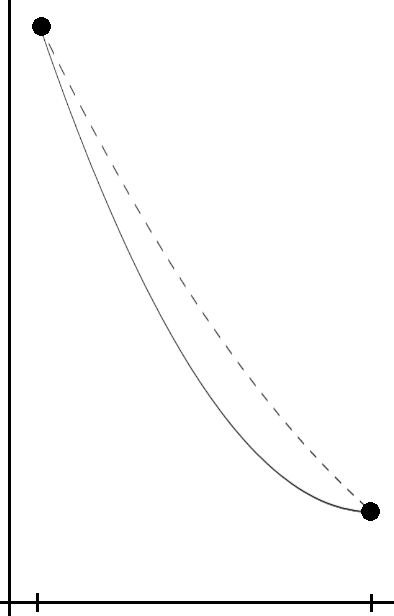
\includegraphics{1}
	\labfig{margin1}
\end{marginfigure}
Definimos $\delta y(x)\equiv\bar{y}(x)-y(x) \label{1.1.1} \inlineeqnum$, donde $\bar{y}$ es el camino variado e $y$ es el camino de referencia. Supondremos que el camino de referencia es el camino que extremiza el funcional, entonces una pequeña variación $\delta y$ no debería alterar el funcional.

Podemos parametrizar $\delta y(x) \equiv a \eta(x) \label{1.1.2} \inlineeqnum$, donde $a$ es un parámetro independiente de $x$ y $\eta(x)=\delta y(x)/a \label{1.1.2} \inlineeqnum$ es una función arbitraria que da forma el camino variado y que debe cumplir que $\eta(x_A)=\eta(x_B)=0 \label{1.1.4} \inlineeqnum$ para verificar las condiciones que hemos impuesto en (1.0.2), ya que todo camino, sea el de referencia o el variado, debe cumplirlas.

Definimos entonces una nueva función $Y(x,a)\equiv y(x)+a\eta(x) \label{1.1.5} \inlineeqnum$ tal que $Y(x,0)=y(x)$ y $Y(x,a)=\bar{y}(x)$. Si derivamos esta función con repecto a $a$, y con respecto a $x$ tenemos
\begin{equation}\label{1.1.6}
\frac{\partial Y}{\partial a}=\eta(x) ; \ \ \frac{\partial Y}{\partial x}=y'(x)+a\eta'(x)\equiv Y'(x,a); \ \  \frac{\partial Y'}{\partial a} = \eta ' (x)
\end{equation} \refstepcounter{subsection}
Podemos definir ahora $\delta y'(x) \equiv \bar{y}'(x)-y'=Y'(x,a)-Y'(x,0)$, que por la expresión anterior nos resulta $\delta y'(x)=a \eta'(x) \label{1.1.7} \inlineeqnum$.
Combinando ahora (1.1.7) y (1.1.2) podemos llegar a la conclusión de que la derivada y $\delta$ conmutan
\begin{equation}\label{1.1.8}
    \delta y'(x)=a \frac{d}{dx} \eta(x)=\frac{d}{dx}\left(a\eta(x)\right)=\frac{d}{dx} \delta y \implies \delta \left(\frac{dy}{dx}\right)=\frac{d}{dx} \delta y 
\end{equation} \refstepcounter{subsection}
%-------------------------------------------------------------------------------------------
\subsection{Variación de una función}
Si partimos de una función $g(y,y';x)$, queremos que no dependa de un solo camino sino de una familia de ellos,  definimos $\mathbb{g}(x,a)=g(Y,Y';x)$. Definimos la variación total de la función como $\Delta \mathbb{g} \equiv \mathbb{g}(Y(x,a),Y'(x,a);x)-\mathbb{g}(Y(x,0),Y'(x,0);x) \label{1.1.9} \inlineeqnum$. Como últimamente $\mathbb{g}$ depende solo de $x$ y de $a$, podemos expandir $\mathbb{g}$ por serie de Taylor de $a$
\begin{equation} \label{1.1.10}
    \mathbb{g}(x,a) = \mathbb{g}(x,0)+\left.\frac{\partial \mathbb{g}}{\partial a}\right|_{a=0} a + O(a^2)
\end{equation} \refstepcounter{subsection}
Reorganizando los términos y volviendo a añadir la dependiencia en $Y$ e $Y'$ llegamos a 
\begin{equation} \label{1.1.11}
    \overbrace{\mathbb{g}(x,a) - \mathbb{g}(x,0) }^{\Delta \mathbb{g}} = \overbrace{\left.\frac{\partial \mathbb{g}(Y(x,a),Y'(x,a);x)}{\partial a}\right|_{a=0} a}^{\delta \mathbb{g}} + O(a^2)
\end{equation} \refstepcounter{subsection}
Donde $\delta \mathbb{g}$ es la variación primera de la función, que podemos reescribir desarrollando la derivada usando la regla de la cadena, y usamos (1.1.2) y (1.1.7)
\begin{equation} \label{1.1.12}
    \delta \mathbb{g}= \left.\left[\left.\frac{\partial \mathbb{g}}{\partial Y}\right|_{Y} \frac{\partial Y}{\partial a} + \left.\frac{\partial \mathbb{g}}{\partial Y'}\right|_{Y} \frac{\partial Y'}{\partial a}\right]\right|_{a=0} a = \left.\frac{\partial \mathbb{g}}{\partial Y}\right|_{y} a \eta + \left.\frac{\partial \mathbb{g}}{\partial Y'}\right|_{y} a \eta' = \left.\frac{\partial \mathbb{g}}{\partial Y}\right|_{y} \delta y + \left.\frac{\partial \mathbb{g}}{\partial Y'}\right|_{y} \delta y'
\end{equation} \refstepcounter{subsection}
Es \textbf{muy} importante no dejar de lado las composiciones y evaluaciones resultantes de hacer Taylor y la regla de la cadena, ya que la expresión anterior nos indica que aunque $g$ dependa de cualquier camino, cuando hacemos $\delta g$, las parciales de $g$ con respecto a sus entradas $Y$ e $Y'$ hay que \textbf{evaluarlas en el camino de referencia} $y=Y(x,0)$. De esta forma podemos reesribir (1.1.12) en términos de $g$
\begin{equation} \label{1.1.12}
    \delta \mathbb{g} = \delta g = \frac{\partial g}{\partial y} \delta y + \frac{\partial g}{\partial y'} \delta y'
\end{equation} \refstepcounter{subsection}
Observamos que nos queda una expresión similar a la regla de la cadena del diferencial exacto de una función.
%-------------------------------------------------------------------------------------------
\subsection{Variación de un funcional}
De nuevo, si partimos de un funcional $F[y]$ que depende de un único camino, definimos $\mathbb{F}([y],a) = F[Y(x,a)]$ y su variación total $\Delta \mathbb{F} = \mathbb{F}([y],a)-\mathbb{F}([y],0) \label{1.1.13} \inlineeqnum$, que desarrollando la integral llegamos inmediatamente a
\begin{equation} \label{1.1.14}
    \Delta \mathbb{F} = \int_{x_A}^{x_B}{\Delta\mathbb{g}dx}=\int_{x_A}^{x_B}{\delta \mathbb{g}dx} + O(a^2)=\underbrace{\int_{x_A}^{x_B}\delta g dx}_{\delta \mathbb{F}=\delta F} + O(a^2)
\end{equation}
\newpage
\section{Extremizar un funcional} \refstepcounter{subsection}
%-------------------------------------------------------------------------------------------
Diremos que el extremo de $F$ ocurrirá cuando $\delta F = 0$, puesto que a primer orden el funcional no cambiará de valor al variar $y$.
De (1.1.13) sustuimos en (1.1.14), sacamos factor común el parámetro $a$ e integramos por partes el segundo término, tal que $ u = \partial_{y'}g$ y $ dv = \eta' dx$
\begin{equation} \label{1.2.1}
    \int_{x_A}^{x_B}{\left[\frac{\partial g}{\partial y} \eta + \frac{\partial g}{\partial y'} \eta'\right] adx} = a \left[\int_{x_A}^{x_B}{\frac{\partial g}{\partial y} \eta dx} + \left|\frac{\partial g}{\partial y'} \eta\right|_{x_A}^{x_B} -\int_{x_A}^{x_B}{\frac{d}{dx}\left(\frac{\partial g}{\partial y'}\right) \eta dx}\right]
\end{equation} \refstepcounter{subsection} 
Por (1.1.4) el segundo término es 0, juntando las integrales y usando (1.1.2)
\begin{equation} \label{1.2.2}
    \int_{x_A}^{x_B}{\left[\frac{\partial g}{\partial y} -\frac{d}{dx}\left(\frac{\partial g}{\partial y'}\right) \right] \delta y dx}=0
\end{equation} \refstepcounter{subsection} 
Ahora, $\delta y$ es completamente arbitrario, pues depende de un parámetro independiente $a$ y de una función $\eta$ que es también arbitraria, esto es lema fundamental del Cálculo Variacional, y garantiza que si la integral debe valer 0, el primer factor debe valer siempre 0, y concluimos

\vspace{-20pt}
\Large\begin{equation} \label{1.2.3}
    \boxed{\frac{\partial g}{\partial y} -\frac{d}{dx}\left(\frac{\partial g}{\partial y'}\right) =0} \iff \delta F =0
\end{equation} \refstepcounter{subsection}\normalsize
Esta es la ecuación de \textit{Euler-Lagrange}, una ecuación diferencial en derivadas parciales de segundo orden cuya solución $y$ extremiza el funcional definido por $g$.

Es importante notar que si definimos
\begin{equation} \label{1.2.2}
    \tilde{g}(f(x),f'(x);x) = g(f(x),f'(x);x) + \frac{d}{dx} h(f(x),x)
\end{equation} \refstepcounter{subsection}
Entonces el funcional nos queda, aplicando el teorema fundamental del cálculo
\begin{equation} \label{1.2.2}
    \tilde{F}[f]=\int_{x_A}^{x_B}{\tilde{g}(f(x),f'(x);x)dx}=F[f] +\int_{x_A}^{x_B}{\frac{d}{dx} h(f(x),x) dx} = F[f] + h(f(x),x)|_{x_A}^{x_B}
\end{equation} \refstepcounter{subsection}
Y como los dos últimos términos son constantes, se verifica que $\delta \tilde{F} = \delta F$, y por lo tanto (1.2.3) permanece invariante bajo esta transformación.
%-------------------------------------------------------------------------------------------
\subsubsection{Geodésica del plano}
Un ejemplo para aplicar (1.2.3) es minimizar la distancia $d=\int{ds}$ en el plano ecuclídeo. Si $y=y(x)$, entonces $ds=\sqrt{dx^2+dy^2}=\sqrt{1+y'^2}dx=g dx$, tal que
\[\frac{\partial g}{\partial y}=0 \implies \frac{d}{dx}\left(\frac{\partial g}{\partial y'}\right)=0 \implies \frac{\partial g}{\partial y'} = \frac{y'}{\sqrt{1+y'^2}}= K \rightarrow y' = \frac{K}{\sqrt{1-K^2}}=\alpha\]
Lo cual implica que $y=\alpha x + y_0$, la ecuación de una recta.
%-------------------------------------------------------------------------------------------
\newpage
\subsection{Identidad de Beltrami}
Podemos reescribir (1.2.3) de otra forma que nos va resultar últil para resolver algunos problemas y va a resultar muy importante en episodios posteriores al definir el \textit{Hamiltoniano}
\[\frac{dg}{dx} = \frac{\partial g}{\partial y} y' + \frac{\partial g}{\partial y'}y'' + \frac{\partial g}{\partial x}\rightarrow \frac{\partial g}{\partial y} y' = \frac{dg}{dx} - \frac{\partial g}{\partial y'}y'' - \frac{\partial g}{\partial x}\]
Podemos observar que el término en el primer miembro de la segunda expresión aparece en (1.2.3) sin multiplicar por $y'$.
\[\frac{dg}{dx} - \frac{\partial g}{\partial x} - \left[\frac{\partial g}{\partial y'}y'' + y' \frac{d}{dx}\left(\frac{\partial g}{\partial y'}\right)\right]=0 \rightarrow \frac{dg}{dx} - \frac{\partial g}{\partial x} - \frac{d}{dx}\left(\frac{\partial g}{\partial y'}y'\right)=0\]
Observando que lo de dentro del paréntesis de la primera expresión es la derivada de un producto, usamos la linearidad de la derivada para obtener
\begin{equation} \label{1.3.4}
    \frac{d}{dx}\left(g -\frac{\partial g}{\partial y'}y'\right)=\frac{\partial g}{\partial x}
\end{equation}
%-------------------------------------------------------------------------------------------

\section{Generalización a varias variables} \refstepcounter{subsection} 
Denotamos $\{f_\alpha(x)\}$ a un conjunto de $N$ funciones distintas, que verifican una expresión similar a (1.0.2), $f_\alpha(x_A)=f_{\alpha A}; \ f_\alpha(x_B)=f_{\alpha B} \label{1.3.1} \inlineeqnum$.
%\sidenote{Si existe una función que las relacione, se trata de una ligadura, veáse el apartado siguiente}
Definimos entonces el siguiente funcional que depende de $\{f_\alpha\}$
\[F[\{f_\alpha\}]=\int_{x_A}^{x_B}{g(\{f_\alpha,f'_\alpha\};x)dx}\]
Ahora siguiendo un desarrollo idéntico a (1.1.12), desarrollando la regla de la cadena para cada una de las variables de $g$ resulta en un sumatorio y los argumentos siguientes para llegar a $\delta g$ son idénticos puesto que son lineales, de tal forma llegamos a la siguiente expresión
\begin{equation} \label{1.3.2}
    \delta g = \sum{\frac{\partial g}{\partial f_\alpha} \delta f_\alpha + \frac{\partial g}{\partial f'_\alpha} \delta f'_\alpha}
\end{equation} \refstepcounter{subsection} 
La expresión (1.1.15) no dependía de las variables de $g$, por lo que es directamente aplicable, sustituyendo (1.3.2) y haciendo la regla de la cadena igual que en (1.2.1) llegamos a una expresión similar a (1.2.2), usando que la integral conmuta con el sumatorio
\begin{equation} \label{1.3.3}
    \delta F = \sum \int_{x_A}^{x_B}{\left[\frac{\partial g}{\partial f_\alpha} -\frac{d}{dx}\left(\frac{\partial g}{\partial f'_\alpha}\right) \right] \delta f_\alpha dx}=0
\end{equation} \refstepcounter{subsection} 
Para poder concluir que cada sumando es 0, y que entonces por ser $\delta f_\alpha$ arbitraria cada término en corchetes es 0, es necesario que los $\delta f_\alpha$ sean independientes entre sí, que es equivalente a que no exista una dependencia explícita entre los $f_\alpha(x)$, que podria estar por ejemplo expresada por una ecuación relacionando varias de ellas. Si se cumple que son independientes, entonces

\vspace{-20pt}
\Large\begin{equation} \label{1.3.3}
    \boxed{\frac{\partial g}{\partial f_\alpha} -\frac{d}{dx}\left(\frac{\partial g}{\partial f'_\alpha}\right) =0} \iff \delta F =0
\end{equation} \refstepcounter{subsection}\normalsize
Ahora tenemos un sistema de ecuaciones de \textit{Euler-Lagrange} cuyas soluciones $f_\alpha(x)$ extremizan el funcional.
%-------------------------------------------------------------------------------------------
\subsection{Ligaduras}
En el caso de que existan $m$ ecuaciones de ligadura de la forma $G_i(\{f_\alpha\};t)=0$, tenemos dos opciones, la primera es resolver el sistema de ecuaciones que forman expresando $m$ funciones como dependientes de las otras $N-m$ funciones restantes, y aplicar (1.3.4) a las $N-m$ funciones independientes.

En el caso de que esto no sea posible resolver el sistema, debemos recurrir a multiplicadores de \textit{Lagrange}.
%-------------------------------------------------------------------------------------------
\subsubsection{Multiplicadores de Lagrange}
Partimos de que tenemos $m$ ecuaciones $G_i(\{f_\alpha\};x)=0$ que no sabemos resolver, $\Delta G_i =0$, es decir, $G_i$ se aplica de la misma forma tanto a los caminos de referencia como a los variados, además $\Delta G_i = \delta G_i + O(a^2) = 0$, como $a$ es arbitrario, entonces $\delta G_i =0$. Aplicando la regla de la cadena de (1.1.13)
\begin{equation} \label{1.3.5}
    \delta G_i(\{f_\alpha\};x) = \sum_\alpha^N{\frac{\partial G_i}{\partial f_\alpha} \delta f_\alpha}=\sum_\alpha^N{a_{i\alpha} \delta f_\alpha}=0; \ \ \ a_{i\alpha} = \frac{\partial G_i}{\partial f_\alpha}
\end{equation} \refstepcounter{subsection}
Así tenemos la ecuación que nos relaciona las distintas $\delta f_\alpha$, el término de la derivada lo podemos expresar como las componentes de un matriz. Podemos separar la expresión anterior tal que
\begin{equation} \label{1.3.6}
    \delta G_i= \sum_{\gamma=1}^{N-m}{a_{i\gamma} \delta f_\gamma} + \sum_{\beta=N-m+1}^{N}{a_{i\beta} \delta f_\beta} = 0
\end{equation} \refstepcounter{subsection}
La matriz del segundo término es cuadrada $(m\times m)$, y es una matriz jacobiana cuyo determinante va a ser no nulo si las ecuaciones de ligadura son independientes entre sí, de lo contrario algunas sobran. Esto implica que esa matriz tiene inversa, expresando (1.3.6) como operaciones matriciales ($N-m < \beta \leq N$)
\begin{equation} \label{1.3.7}
    0= A\mathbf{x} + J\mathbf{y} \implies \mathbf{y}=-J^{-1}A\mathbf{x}; \ \ \delta f_\beta = -\sum_{a=1}^m{\sum_{\gamma =1}^{N-m}{J^{-1}_{\beta a}a_{a\gamma}\delta f_\gamma}}
\end{equation} \refstepcounter{subsection}
De esta forma, hemos encontrado la dependencia explícita de $\delta f_\beta$ en función de los $\delta f_\gamma$, estos últimos siendo independientes entre sí. Ahora tomamos (1.3.3) y renombramos el factor en corchetes por $\Gamma_\alpha$ y separamos como en (1.3.6)
\begin{equation} \label{1.3.8}
    0 = \delta F = \int_{x_A}^{x_B}{\sum_\alpha^N{(\Gamma_\alpha \delta f_\alpha)}dx=\int_{x_A}^{x_B}{\sum_{\gamma =1}^{N-m}{(\Gamma_\gamma \delta f_\gamma)}dx+\int_{x_A}^{x_B}{\sum_{\beta=N-m+1}^{N}{(\Gamma_\beta \delta f_\beta)}dx}}}
\end{equation} \refstepcounter{subsection}
Sustituyendo $\delta f_\beta$ de (1.3.7)
\begin{equation} \label{1.3.9}
    0 =\int_{x_A}^{x_B}{\sum_{\gamma =1}^{N-m}{(\Gamma_\gamma \delta f_\gamma)}dx-\int_{x_A}^{x_B}{\sum_{\beta=N-m+1}^{N}{\left(\Gamma_\beta \sum_{a=1}^m{\sum_{\gamma =1}^{N-m}{J^{-1}_{\beta a}a_{a\gamma}\delta f_\gamma}}\right)}dx}}
\end{equation} \refstepcounter{subsection}
Como los sumatorios conmutan podemos llegar a
\begin{equation} \label{1.3.10}
    0  =\int_{x_A}^{x_B}{\sum_{\gamma =1}^{N-m}{(\Gamma_\gamma \delta f_\gamma)}dx-\int_{x_A}^{x_B}\sum_{\gamma =1}^{N-m}{{\sum_{a=1}^m{\sum_{\beta=N-m+1}^{N}{\Gamma_\beta J^{-1}_{\beta a}a_{a\gamma}\delta f_\gamma}}}dx}}
\end{equation} \refstepcounter{subsection} 
Y ahora podemos unificar los sumatorios de $\gamma$ y sacar factor común $\delta f_\gamma$
\begin{equation} \label{1.3.11}
    0  =\int_{x_A}^{x_B}{\sum_{\gamma =1}^{N-m}{\delta f_\gamma \left(\Gamma_\gamma -{\sum_{a=1}^m{\sum_{\beta=N-m+1}^{N}{\Gamma_\beta J^{-1}_{\beta a}a_{a\gamma}}}}\right)} dx}
\end{equation} \refstepcounter{subsection} 
Definimos entonces $\lambda_a=\sum_{\beta=N-m+1}^{N}{\Gamma_\beta J^{-1}_{\beta a}}$ como los multiplicadores de \textit{Lagrange} y reemplazando $a_{a\gamma}$ por su definición de (1.3.5)
\begin{equation} \label{1.3.12}
    0  =\int_{x_A}^{x_B}{\sum_{\gamma =1}^{N-m}{\delta f_\gamma \left(\Gamma_\gamma -{\sum_{a=1}^m{\lambda_a \frac{\partial G_a}{\partial f_\gamma}}}\right)} dx}
\end{equation} \refstepcounter{subsection}
Ahora como $\delta f_\gamma$ son independientes entre sí, podemos aplicar el mismo argumento que en los otros casos y concluir que lo del paréntesis debe ser igual a 0 para todos los $\gamma$, tal que ($1 \leq \gamma \leq N-m$)
\begin{equation} \label{1.3.13}
    \Gamma_\gamma -{\sum_{a=1}^m{\lambda_a \frac{\partial G_a}{\partial f_\gamma}}}=0
\end{equation} \refstepcounter{subsection}
Podemos ahora comprobar que si $N-m < \gamma \leq N$
\[\Gamma_\gamma -{\sum_{a=1}^m{\lambda_a \frac{\partial G_a}{\partial f_\gamma}}}\right)=\Gamma_\gamma -{\sum_{a=1}^m{\lambda_a J_{a\gamma}}}\right) = \Gamma_\gamma -{\sum_{a=1}^m{\sum_{\beta=N-m+1}^{N}{\Gamma_\beta J^{-1}_{\beta a}} J_{a\gamma}}}=\]
\begin{equation} \label{1.3.14}
    =\Gamma_\gamma -\sum_{\beta=N-m+1}^{N}{\Gamma_\beta \delta_{\beta \gamma}} \right) = \Gamma_\gamma - \Gamma_\gamma = 0
\end{equation} \refstepcounter{subsection}
También se verifica (1.3.12), por lo que entonces
\Large\begin{equation} \label{1.3.15}
    \boxed{\frac{\partial g}{\partial f_\alpha} -\frac{d}{dx}\left(\frac{\partial g}{\partial f'_\alpha}\right) ={\sum_{i=1}^m{\lambda_i \frac{\partial G_i}{\partial f_\alpha}}} \ \ \ \ \ G_i(\{f_\alpha\}) = 0}
\end{equation} \refstepcounter{subsection}\normalsize
Tenemos por lo tanto un sistema de $N+m$ ecuaciones, que incluye las ecuaciones de \textit{Euler-Lagrange} modificadas y las ecuaciones de ligadura, y las incognitas son las $f_\alpha$ y las $\lambda_i$.
\chapter{Mecánica Lagrangiana}
\labch{intro}
%-------------------------------------------------------------------------------------------
Ahora la variable independiente sobre la que vamos a trabajar va a ser el tiempo, $t$, y las variables dependientes son las coordenadas cartesianas $\{x_{\alpha i}\}$, donde $\alpha$ indica la partícula y $i$ indica la componente de la posición.
Definimos además las derivadas totales temporales como $\{\dot{x}_{\alpha i}\}$.

\section{Principio de Hamilton}\refstepcounter{subsection}

Definimos una función llamada \textbf{Lagrangiano}\sidenote{La definición de \textbf{Lagrangiano} dependerá de la configuración del sistema físico, pero como norma géneral en mecánica clásica (2.1.1) es la expresión más común de la función que verifica (2.1.3). Esto se demuestra más adelante.}
\begin{equation} \label{2.1.1}
    \pazocal{L}(\{x_{\alpha i},\dot{x}_{\alpha i}\};t)=T-U
\end{equation} \refstepcounter{subsection}
Dónde $T$ es la energía cinética del sistema y $U$ es la energía potencial (conservativa o no), de tal forma que definimos el siguiente funcional llamado \textbf{acción}
\begin{equation} \label{2.1.2}
    S \equiv \int_{t_A}^{t_B}{\pazocal{L}(\{x_{\alpha i},\dot{x}_{\alpha i}\};t)dt}
\end{equation} \refstepcounter{subsection}
\textbf{Principio de Hamilton o de mínima acción.} La evolución temporal de un sistema físico es aquella que extremiza la acción, es decir que $\delta S = 0$ para la evolución real del sistema, lo cual es equivalente a
\begin{equation} \label{2.1.3}
    \frac{\partial \pazocal{L}}{\partial x_{\alpha i}} -\frac{d}{dt}\left(\frac{\partial \pazocal{L}}{\partial \dot{x}_{\alpha i}}\right) =0
\end{equation} \refstepcounter{subsection}
Para la mecánica clásica, este principio es equivalente a las leyes de \textit{Newton}, cuando $\pazocal{L}$ toma la forma de (2.1.1) con ligeras modificaciones que discutiremos en las próximas secciones.
%-------------------------------------------------------------------------------------------
\subsubsection{Muelle elástico}
Un sencillo ejemplo para aplicar este principio es el de un muelle elástico en una dirección, donde $T=m\dot{x}^2/2$ y $U = kx^2/2$ (el término $mgh$ es constante y puede ser ignorado), si $\pazocal{L} = T-U$, entonces
\[\frac{\partial \pazocal{L}}{\partial x}=-kx \ \ \ \ \frac{\partial \pazocal{L}}{\partial \dot{x}}=m\dot{x} = p \ \ \ \ \frac{d p}{dt} = m\ddot{x} \rightarrow m\ddot{x} = -kx \iff F=-kx=ma\]
%-------------------------------------------------------------------------------------------
\section{Coordendas generalizadas} \refstepcounter{subsection}
Podemos realizar un cambio de variables para poder expresar $x_{\alpha i}$ en función de otras variables $q_j$, las cuales pueden resultarnos más sencillas para resolver un problema, tal que $x_{\alpha i}=x_{\alpha i}(\{q_j\};t)$. Esta transformación será invertible cuando
\vspace{-10pt}
\[J_l^k=\frac{\partial x_k}{\partial q_l}\]
el determinante de esa matriz, el jacobiano, sea no nulo, tal que existe la transformación $q_j = q_j(\{x_{\alpha i}\};t)$.

Usando la regla de la cadena podemos ver la dependencia de las velociades entre sí, $\dot{x}_{\alpha i}=\dot{x}_{\alpha i}(\{q_j,\dot{q}_j\};t)$ y que $\dot{q}_j = \dot{q}_j(\{x_{\alpha i},\dot{x}_{\alpha i}\};t)$.

De esta forma, podemos expresar $\pazocal{L}$ en función de las coordenadas y velocidades generalizadas, tal que $\pazocal{L}=\pazocal{L}(\{q_j,\dot{q}_j\};t)$ de tal forma que (2.1.3) queda como 

\vspace{-10pt}
\Large\begin{equation} \label{2.2.1}
    \boxed{\frac{\partial \pazocal{L}}{\partial q_j} -\frac{d}{dt}\left(\frac{\partial \pazocal{L}}{\partial \dot{q}_j}\right) =0}
\end{equation} \refstepcounter{subsection}\normalsize

Definimos además el \textbf{momento generalizado}, que para cartesianas es el momento lineal y para polares es el momento angular. También definimos la \textbf{fuerza generalizada}, que es la proyección del vector cartesiano en el sistema de vectores asociado a las coordenadas generalizadas.
\begin{equation} \label{2.2.2}
    p_j = \frac{\partial \pazocal{L}}{\partial \dot{q}_j} \ \ \ \ Q_j = -\frac{\partial U}{\partial q_j}=\sum_\alpha^N{\mathbf{F}_\alpha\cdot \frac{\partial \mathbf{r}_{\alpha}}{\partial q_j}}
\end{equation} \refstepcounter{subsection}
%-------------------------------------------------------------------------------------------
\section{Ligaduras}\refstepcounter{subsection}
Al igual que en la sección \textit{Ligaduras} de la sección 1.3, tendremos $M$ ecuaciones de ligadura, los tipos de las cuales se datallarán a continuación, pero antes definimos lo que vamos a denominar \textbf{grados de libertad}, que indica el número mínimo de parámetros que es necesario para especifcar la configuración del sistema en un tiempo dado, tal que $s = N\cdot d- M \label{2.3.1} \inlineeqnum$, donde $s$ son los \textbf{grados de libertad}, $N$ el número de partículas del sistema, y $d$ la dimensión del espacio.
%-------------------------------------------------------------------------------------------
\subsubsection{Tipos de ligaduras}
Cuando las ecuaciones de ligadura no dependen de las veclocidades, $G_i(\{q_j\})=0$, se denominan ligaduras \textbf{holónomas} y son con las que vamos a trabajar. Si las ecuaciones de ligadura dependen de la velocidad,$ G_i(\{q_j,\dot{q}_j\})=0$, se denominan \textbf{no holónomas} y salvo que sean integrables no trabjaremos con ellas. Son \textbf{integrables} cuando son de la forma siguiente donde $h=h(\{q_i\};t)$ tal que
\begin{equation} \label{2.3.2}
    \sum_j^{N\cdot d}{A_j(\{q_i\};t)\dot{q}_j} + B(\{q_i\};t)=0; \ \ \ \ A_j=\frac{\partial h}{\partial q_j}; \ \ \ \ B_j=\frac{\partial h}{\partial t}
\end{equation} \refstepcounter{subsection}
Entonces podemos ver que nos queda la regla de la cadena e integramos
\begin{equation} \label{2.3.3}
    \sum_j^{N\cdot d}{\frac{\partial h}{\partial q_j}\dot{q}_j} + \frac{\partial h}{\partial t}=\frac{d h}{dt} =0 \iff h(\{q_i\};t) - C = 0 \mbox{ (Holónoma)}
\end{equation} \refstepcounter{subsection}
Luego a parte si la ligadura depende explícitamente del tiempo se llama \textbf{forzada} o \textbf{reónoma}, si no depende explcítamente del tiempo, se denominan \textbf{naturales} o \textbf{esclerónomas}.
%-------------------------------------------------------------------------------------------
\subsection{Sistema holonómico}
Decimos que un sistema es \textbf{holonómico} cuando podemos resolver (o bien en cartesianas o en generalizadas) las ecuaciones de ligadura (holónomas) y expresar $m$ coordenadas como explícitamente dependientes de $s$ coordenadas independientes, reduciendo el sistema a $s$ variables que podemos resolver usando (2.2.1)  (\textit{E-L}).
%-------------------------------------------------------------------------------------------
\subsection{Multiplicadores de Lagrange}
En el caso en el que el sistema no sea holonómico, y no podamos resolver las ecuaciones de ligadura, al igual que en la sección 1.3 tenemos que recurrir a multiplicadores de multiplicadores de \textit{Lagrange}, podemos obtener una expresión equivalente a (1.3.15) modificando el lagrangiano de la siguiente forma
\begin{equation} \label{2.3.4}
    \pazocal{L}^* = \pazocal{L}+\sum^m{\lambda_i G_i}
\end{equation} \refstepcounter{subsection}
Que aplicando las ecuaciones de \textit{Euler-Lagrange} tanto para $q_j$ como para $\lambda_i$ resulta

\vspace{-10pt}
\Large\begin{equation} \label{2.3.5}
    \frac{\partial \pazocal{L}}{\partial q_j} -\frac{d}{dt}\left(\frac{\partial \pazocal{L}}{\partial \dot{q}_j}\right) +\underbrace{\sum^m\lambda_i(t)\frac{\partial G_i}{\partial q_j}}_{Q^L_j}=0
\end{equation} \refstepcounter{subsection}\normalsize
Donde $Q^L_j$ es la componente $j$ de la fuerza generalizada de ligadura total, que cumplen que $dW^L = \mathbf{F}^L\cdot d\mathbf{r}=0$ son fuerzas que o siempre perpendiculares a la ligadura, o que provocan que $d\mathbf{r}=0 \iff \mathbf{v}=0$ en el punto de contacto.

\section{Principio de D'Alambert}\refstepcounter{subsection}
\subsubsection{Estático}
Vamos a suponer que tenemos un sistema en equilibrio, es decir $\mathbf{F}_i = 0$ para cada partícula del sistema, o en general para cualquier punto donde se aplica una fuerza, de tal forma que $\mathbf{F}_i \cdot \delta \mathbf{r}_i = 0$.

$\delta \mathbf{r}_i$ es lo que se denomina desplazamiento virtual, el sistema no se mueve, sigue en el equilibrio, estos desplazamientos se definen respetando las ligaduras del sistema, por ejemplo, tenemos en un péndulo que por la gravedad y otra fuerza externa se encuentra en equilibrio, podemos expresar la posición en términos de las coordenadas generalizadas, que respetan las ligaduras, tal que $\mathbf{r} = l (\sin \theta \mathbf{e}_x + \cos \theta \mathbf{e}_y)$, y entonces $\delta \mathbf{r} = l (\cos \theta \mathbf{e}_x-\sin\theta \mathbf{e}_y) \delta \theta$.

Para sistemas tendremos entones $\sum_i \mathbf{F}_i \cdot \delta \mathbf{r}_i = 0$, pero esto no nos dice nada, sin embargo, podemos descomponer la fuerza total que se ejerce en un punto o partícula en fuerzas de ligadura o normal y fuerzas externas o aplicadas, tal que $\mathbf{F}_i = \mathbf{F}_i^{(a)}+\mathbf{f}_i$, aunque no es siempre facil distinguirlo a simple vista. De esta forma nos queda
\begin{equation} \label{2.1.1}
    \sum_i \mathbf{F}_i^{(a)} \cdot \delta \mathbf{r}_i + \sum_i \mathbf{f}_i \cdot \delta \mathbf{r}_i = 0
\end{equation} \refstepcounter{subsection}
Ahora, salvo casos muy extraños de ligaduras, el trabajo virtual de una fuerza normal o de ligadura se anula, como se ha explicado en el apartado anterior, de esta forma llegamos al principio de D'Alambert estático
\begin{equation} \label{2.1.1}
    \sum_i \mathbf{F}_i^{(a)} \cdot \delta \mathbf{r}_i = 0
\end{equation} \refstepcounter{subsection}
También es llamado principio del trabajo virtual, y al aplicarlo, las componentes $\delta \mathbf{r}_i$ son no nulas, en general implica que $\delta q_i \neq 0$, donde $q_i$ son las coordenadas generalizadas, por ejemplo, $\delta \theta$ en el ejemplo anterior.
\subsubsection{Dinámico}
Ahora consideraremos un sistema que no esta en equilibrio, tenemos que $\mathbf{F}_i = \dot{\mathbf{p}}_i = m_i \ddot{\mathbf{r}}_i$, de tal forma que haciendo exactamente las mismas manipulaciones que antes, y descomponiendo la fuerza total, llegamos a la versión dinámica del principio de D'Alambert
\begin{equation} \label{2.1.1}
    \sum_i (\dot{\mathbf{p}}_i-\mathbf{F}_i^{(a)}) \cdot \delta \mathbf{r}_i = 0
\end{equation} \refstepcounter{subsection}
\subsubsection{Lagrangiano}
Si hacemos el cambio a coordenadas generalizadas usando la regla de la cadena, tenemos
\begin{equation} \label{2.1.1}
    \delta \mathbf{r}_i = \sum_j \frac{\partial \mathbf{r}_i}{\partial q_j} \delta q_j
\end{equation} \refstepcounter{subsection}
Podemos ahora definir de nuevo la fuerza generalizada
\begin{equation} \label{2.1.1}
    \sum_i \mathbf{F}_i \cdot \delta \mathbf{r}_i = \sum_{ij} \mathbf{F}_i \cdot \frac{\partial \mathbf{r}_i}{\partial q_j} \delta q_j = \sum_j Q_j \delta q_j \implies Q_j = \sum_i \mathbf{F}_i \cdot \frac{\partial \mathbf{r}_i}{\partial q_j}
\end{equation} \refstepcounter{subsection}
Es importante notar que $Q_j$ no tiene unidades de fuerza en general, pero $Q_j \delta q_j$ siempre tiene unidades de trabajo. Si consideramos solo fuerzas conservativas (aunque pueden depender del tiempo) tenemos
\begin{equation} \label{2.1.1}
    \mathbf{F}_i = -\nabla_i U \ \ \ \ \ \ Q_j = -\sum_i \nabla_i U \cdot \frac{\partial \mathbf{r}_i}{\partial q_j} = - \sum_{ik} \frac{\partial U}{\partial r_{ik}} \frac{\partial r_{ik}}{\partial q_j} = - \frac{\partial U}{\partial q_j}
\end{equation} \refstepcounter{subsection}
Ahora, hacemos lo mismo pero con el otro término de (2.4.3), y descomponemos una regla del producto
\begin{equation} \label{2.1.1}
    \sum_i \dot{\mathbf{p}}_i \cdot \delta \mathbf{r}_i = \sum_{ij} m \ddot{\mathbf{r}}_i \cdot \frac{\partial \mathbf{r}_i}{\partial q_j} \delta q_j \ \ \ \ \ \ \ \sum_{i} m \ddot{\mathbf{r}}_i \cdot \frac{\partial \mathbf{r}_i}{\partial q_j} = \sum_i \left[ \frac{d}{dt}\left(m_i \dot{\mathbf{r}}_i \cdot \frac{\partial \mathbf{r}_i}{\partial q_j}\right)- m_i \dot{\mathbf{r}}_i\frac{d}{dt}\left(\frac{\partial \mathbf{r}_i}{\partial q_j}\right)\right]
\end{equation} \refstepcounter{subsection}
\begin{equation} \label{2.1.1}
    \frac{d}{dt}\left(\frac{\partial \mathbf{r}_i}{\partial q_j}\right) = \sum_k \frac{\partial^2 \mathbf{r}_i}{\partial q_j \partial q_k}\dot{q}_k + \frac{\partial^2 \mathbf{r}_i}{\partial q_j \partial t} = \frac{\partial}{\partial q_j}\left( \sum_k \frac{\partial \mathbf{r}_i}{ \partial q_k}\dot{q}_k + \frac{\partial\mathbf{r}_i}{\partial t} \right)= \frac{\partial \dot{\mathbf{r}}_i}{\partial q_j} = \frac{\partial \mathbf{v}_i}{\partial q_j}
\end{equation} \refstepcounter{subsection}
Además podemos ver que
\begin{equation} \label{2.1.1}
    \frac{\partial \mathbf{v}_i}{\partial \dot{q}_j} = \frac{\partial}{\partial \dot{q}_j}\left( \sum_k \frac{\partial \mathbf{r}_i}{ \partial q_k}\dot{q}_k + \frac{\partial\mathbf{r}_i}{\partial t} \right) = \sum_k \frac{\partial \mathbf{r}_i}{ \partial q_k} \delta_{kj} =  \frac{\partial \mathbf{r}_i}{ \partial q_j}
\end{equation} \refstepcounter{subsection}
Ahora, introducimos (2.4.7) en (2.4.6) tal que
\[\sum_i \dot{\mathbf{p}}_i \cdot \delta \mathbf{r}_i = \sum_{ij} \left[ \frac{d}{dt}\left(m_i \mathbf{v}_i \cdot \frac{\partial \mathbf{v}_i}{\partial \dot{q}_j}\right)- m_i \mathbf{v}_i\frac{\partial \mathbf{v}_i}{\partial q_j}\right] \delta q_j = \]
\begin{equation} \label{2.1.1}
     = \sum_{ij} \left[ \frac{d}{dt}\left(\frac{\partial}{\partial \dot{q}_j} \left(\frac{1}{2}m_i \mathbf{v}_i \cdot \mathbf{v}_i\right)\right)- \frac{\partial}{\partial q_j} \left(\frac{1}{2}m_i \mathbf{v}_i \cdot \mathbf{v}_i\right)\right] \delta q_j = \sum_{j} \left[ \frac{d}{dt}\left(\frac{\partial T}{\partial \dot{q}_j}\right)- \frac{\partial T}{\partial q_j}\right] \delta q_j
\end{equation} \refstepcounter{subsection}
Ahora metiendo (2.4.10) y (2.4.6) en (2.4.3)
\begin{equation} \label{2.1.1}
    \sum_{j} \left[ \frac{d}{dt}\left(\frac{\partial T}{\partial \dot{q}_j}\right)- \frac{\partial T}{\partial q_j} +\frac{\partial U}{\partial q_j}\right] \delta q_j = 0
\end{equation} \refstepcounter{subsection}
Ahora, si suponemos que tenemos un sistema holonómico y que podemos resolver las ligaduras y que $q_j$ son holónomas, y por lo tanto independientes, y a du vez $\delta q_j$ también, tenemos el siguiente conjunto de ecuaciones
\begin{equation} \label{2.1.1}
    \frac{d}{dt}\left(\frac{\partial (T-U)}{\partial \dot{q}_j}\right)-\frac{\partial (T-U)}{\partial q_j} = 0 \ \ \ \ \ \ T-U= \pazocal{L}
\end{equation} \refstepcounter{subsection}
Como estamos considerando fuerzas conservativas, sus potenciales no dependen de las velocidades generalizadas, y por lo tanto la podemos introducir en el primer término de la ecuación sin pérdida de generalidad, y voalá, hemos demostrado (2.1.2), el principio de Hamilton para la mecánica de Newton bajo unos ciertos supuestos.

Podemos considerar fuerzas no conservativas, como por ejemplo, un rozamiento dinámico, separandolas, tal que
\begin{equation} \label{2.1.1}
    Q_j = - \frac{\partial U}{\partial q_j} + \sum \mathbf{F}^{(nc)} \cdot \frac{\partial \mathbf{r}_i}{\partial q_j} = - \frac{\partial U}{\partial q_j} + Q_j^{(nc)} \implies \frac{d}{dt}\left(\frac{\partial \pazocal{L}}{\partial \dot{q}_j}\right)-\frac{\partial \pazocal{L}}{\partial q_j} =  Q_j^{(nc)}
\end{equation} \refstepcounter{subsection}
\subsubsection{Potencial generalizado}
Además, podemos crear un tipo de potencial generalizado que dependa de $\dot{q}_j$, para ello, primero tomamos la forma genérica de (2.4.11) sin asumir nada sobre la fuerza
\begin{equation} \label{2.1.1}
    \frac{d}{dt}\left(\frac{\partial T}{\partial \dot{q}_j}\right)-\frac{\partial T}{\partial q_j} = Q_j
\end{equation} \refstepcounter{subsection}
Y por otro lado descomponemos la parte cinética y potencial de (2.4.12) e igualamos
\begin{equation} \label{2.1.1}
    \frac{d}{dt}\left(\frac{\partial U}{\partial \dot{q}_j}\right)-\frac{\partial U}{\partial q_j} = Q_j = \sum_i \mathbf{F}_i \cdot \frac{\partial \mathbf{r}_i}{\partial q_j}
\end{equation} \refstepcounter{subsection}
Entonces cualquier fuerza que pueda ser derivada de un potencial $U(\{q_i\},\{\dot{q}_i\})$ (no puede depender del tiempo en este caso) siguiendo (2.4.15) verifica también el principio de Hamilton.

El ejemplo más notable de este tipo de potencial es el que crea la fuerza electromagnética, vamos a estudiarlo, lo primero es saber que es $Q_j$ en este caso, usaremos coordenadas cartesianas
\begin{equation} \label{2.1.1}
    Q_j = \sum_i \mathbf{F}_i \cdot \frac{\partial \mathbf{r}_i}{\partial x_j} = \sum_i \mathbf{F}_i \cdot \mathbf{e}_i \delta_{ij} = F_j
\end{equation} \refstepcounter{subsection}
La fuerza de Lorentz es, y podemos definir los campos $\mathbf{E}$ y $\mathbf{B}$ como 
\begin{equation} \label{2.1.1}
    \mathbf{F}(\mathbf{r},\dot{\mathbf{r}}) = q(\mathbf{E}(\mathbf{r})+\dot{\mathbf{r}} \times \mathbf{B}(\mathbf{r})) \ \ \ \ \ \ \ \mathbf{E}(\mathbf{r}) = -\nabla_\mathbf{r} \phi -\frac{\partial \mathbf{A}}{\partial t}  \ \ \ \ \ \ \ \mathbf{B}(\mathbf{r}) = \nabla_\mathbf{r} \times \mathbf{A}
\end{equation} \refstepcounter{subsection}
\[
    B_x = \partial_y A_z - \partial_z A_y \ \ \ \ \ B_y = \partial_z A_x-\partial_x A_z \ \ \ \ \ B_z = \partial_x A_y - \partial_y A_x
\]
\[
    (\dot{\mathbf{r}} \times \mathbf{B})_x= \dot{y}B_z - \dot{z}B_y \ \ \ \ \ (\dot{\mathbf{r}} \times \mathbf{B})_y = \dot{z}B_x - \dot{x}B_z \ \ \ \ \ (\dot{\mathbf{r}} \times \mathbf{B})_z = \dot{x}B_y - \dot{y}B_x
\]
\[F_x = q\left(-\partial_x \phi - \partial_t A_x +\dot{y}B_z - \dot{z}B_y\right) = q\left(-\partial_x \phi - \partial_t A_x +\dot{y}(\partial_x A_y - \partial_y A_x) - \dot{z}(\partial_z A_x-\partial_x A_z)\right)\]
\[F_y = q\left(-\partial_y \phi - \partial_t A_y +\dot{z}B_x - \dot{x}B_z\right) = q\left(-\partial_y \phi - \partial_t A_y +\dot{z}(\partial_y A_z - \partial_z A_y) - \dot{x}(\partial_x A_y-\partial_y A_x)\right)\]
\[F_z = q\left(-\partial_z \phi - \partial_t A_z +\dot{x}B_y - \dot{y}B_x\right) = q\left(-\partial_z \phi - \partial_t A_z +\dot{x}(\partial_z A_x-\partial_x A_z) - \dot{y}(\partial_y A_z - \partial_z A_y)\right)\]
\[F_x = \frac{d}{dt}\left(\frac{\partial U}{\partial \dot{x}}\right)-\frac{\partial U}{\partial x} = \frac{\partial^2 U}{\partial \dot{x}\partial x} \dot{x} + \frac{\partial^2 U}{\partial \dot{x}\partial y} \dot{y} + \frac{\partial^2 U}{\partial \dot{x}\partial z} \dot{z} + \frac{\partial^2 U}{\partial^2 \dot{x}} \ddot{x} + \frac{\partial^2 U}{\partial \dot{x}\partial \dot{y}} \ddot{y} + \frac{\partial^2 U}{\partial \dot{x}\partial \dot{z}} \ddot{z}+\frac{\partial^2 U}{\partial \dot{x}\partial t} -\frac{\partial U}{\partial x}\]
\[F_y = \frac{d}{dt}\left(\frac{\partial U}{\partial \dot{y}}\right)-\frac{\partial U}{\partial y} = \frac{\partial^2 U}{\partial \dot{y}\partial x} \dot{x} + \frac{\partial^2 U}{\partial \dot{y}\partial y} \dot{y} + \frac{\partial^2 U}{\partial \dot{y}\partial z} \dot{z} + \frac{\partial^2 U}{\partial \dot{y} \partial \dot{x}} \ddot{x} + \frac{\partial^2 U}{\partial^2 \dot{y}} \ddot{y} + \frac{\partial^2 U}{\partial \dot{y}\partial \dot{z}} \ddot{z}+\frac{\partial^2 U}{\partial \dot{y}\partial t} -\frac{\partial U}{\partial y}\]
\[F_z = \frac{d}{dt}\left(\frac{\partial U}{\partial \dot{z}}\right)-\frac{\partial U}{\partial z} = \frac{\partial^2 U}{\partial \dot{z}\partial x} \dot{x} + \frac{\partial^2 U}{\partial \dot{z}\partial y} \dot{y} + \frac{\partial^2 U}{\partial \dot{z}\partial z} \dot{z} + \frac{\partial^2 U}{\partial \dot{z}\partiañ \dot{x}} \ddot{x} + \frac{\partial^2 U}{\partial \dot{z}\partial \dot{y}} \ddot{y} + \frac{\partial^2 U}{\partial^2 \dot{z}} \ddot{z}+\frac{\partial^2 U}{\partial \dot{z}\partial t} -\frac{\partial U}{\partial z}\]
Lo términos de $\ddot{q}$ no aparecen, por lo que $U$ debe ser lineal en $\dot{q}$, gracias a los dos últimos términos, podemos integrar y saber que al menos
\begin{equation} \label{2.1.1}
    U = q(\phi -\dot{\mathbf{r}}\cdot \mathbf{A})
\end{equation} \refstepcounter{subsection}
Hace encajar los términos eléctricos $ q(-\partial_i \phi - \partial_t A_i)$, pero es que además, si sustituimos en el resto de términos, también se cumple para los términos magnéticos.
Hay muchas manipulaciones que se pueden hacer para ver esto más sencillo, por ejemplo, usando relaciones vectoriales.
%-------------------------------------------------------------------------------------------
\section{Teorema de la Energía Cinética}\refstepcounter{subsection}
%-------------------------------------------------------------------------------------------
\subsection{Función k-homogénea}
Una función k-homogéna cumple la siguiente expresión, donde $\lambda$ es un parámetro arbitrario cualquiera
\begin{equation} \label{2.4.1}
    f(\{\lambda x_i\})=\lambda^k f(\{x_i\})
\end{equation} \refstepcounter{subsection}
\vspace{-35pt}
\subsubsection{Teorema de Euler}
Podemos derivar cada lado de (2.4.1) con respecto al parámetro
\[\frac{\partial}{\partial \lambda} f(\{\lambda x_i\})= \frac{\partial}{\partial \lambda} \lambda^k f(\{x_i\})\]
En el primer miembro hacemos la regla de la cadena y en el segundo es la derivada de una potencia
\[\sum_j^N \frac{\partial f(\{\lambda x_i\})}{\partial (\lambda x_j)} \frac{d (\lambda x_j)}{d \lambda}= \sum_j^N \frac{\partial f(\{\lambda x_i\})}{\partial (\lambda x_j)} x_j=  k \lambda^{k-1} f(\{x_i\})\]
Como $\lambda$ es un parámetro arbitrario, podemos tomar $\lambda=1$ y tenemos
\begin{equation} \label{2.4.2}
    \sum_j^N \frac{\partial f(\{x_i\})}{\partial x_j} x_j=  k f(\{x_i\})
\end{equation} \refstepcounter{subsection}
%------------------------------------------------------------------------------------------
\subsection{Forma cuadrática}
Una forma cuadrática es una función 2-homogénea de la siguiente forma
\begin{equation} \label{2.4.3}
    f(\{x_i\})=\sum_{i,j}^N{{a_{jk} x_j x_k}}=\mathbf{x} A \mathbf{x}^T
\end{equation} \refstepcounter{subsection}
Donde $a_{jk}$ no tienen por que ser constantes, pueden ser funciones de otras variables, pero no de $x_i$.
%------------------------------------------------------------------------------------------
\subsection{Teorema}
En coordenadas cartesianas la expresión de la energía cinética es una forma cuadrática que solo depende de las velocidades que tiene la siguiente forma
\begin{equation} \label{2.4.4}
    T=T(\{x_{\alpha i}\})=\frac{1}{2} \sum_{\alpha, i}^{N,d} m_\alpha \dot{x}_{\alpha i}^2
\end{equation} \refstepcounter{subsection}
\vspace{-25pt}

Si $x_{\alpha i}(\{q_j\};t)$, entonces
\begin{equation} \label{2.4.5}
    \dot{x}_{\alpha i}=\sum_j^s \frac{\partial x_{\alpha i}}{\partial q_j}\dot{q}_j + \frac{\partial x_{\alpha i}}{\partial t}=\dot{x}_{\alpha i}(\{q_j,\dot{q}_j\};t)
\end{equation} \refstepcounter{subsection}
Elevando (2.4.5) al cuadrado tenemos
\[\dot{x}_{\alpha i}^2= \left(\sum_j^s \frac{\partial x_{\alpha i}}{\partial q_j}\dot{q}_j \right) \left(\sum_k^s \frac{\partial x_{\alpha i}}{\partial q_k}\dot{q}_k \right) + 2\frac{\partial x_{\alpha i}}{\partial t} \sum_j^s \frac{\partial x_{\alpha i}}{\partial q_j}\dot{q}_j  + \left(\frac{\partial x_{\alpha i}}{\partial t}\right)^2 = \]
\begin{equation} \label{2.4.6}
    = \sum_{j,k}^s{\frac{\partial x_{\alpha i}}{\partial q_j}\frac{\partial x_{\alpha i}}{\partial q_k}\dot{q}_j\dot{q}_k} + 2\frac{\partial x_{\alpha i}}{\partial t} \sum_j^s \frac{\partial x_{\alpha i}}{\partial q_j}\dot{q}_j + \left(\frac{\partial x_{\alpha i}}{\partial t}\right)^2
\end{equation} \refstepcounter{subsection}
Sustituyendo (2.4.6) en (2.4.4)
\[ T = \frac{1}{2} \sum_{\alpha, i}^{N,d} m_\alpha \left[\sum_{j,k}^s{\frac{\partial x_{\alpha i}}{\partial q_j}\frac{\partial x_{\alpha i}}{\partial q_k}\dot{q}_j\dot{q}_k} + 2\frac{\partial x_{\alpha i}}{\partial t} \sum_j^s \frac{\partial x_{\alpha i}}{\partial q_j}\dot{q}_j + \left(\frac{\partial x_{\alpha i}}{\partial t}\right)^2\right]\]
Usando que los sumatorios conmutan y son lineales llegamos a
\begin{equation}  
    T = \sum_{j,k}^s{\left(\sum_{\alpha,i}^{N,d}{ \frac{1}{2} m_\alpha \frac{\partial x_{\alpha i}}{\partial q_j}\frac{\partial x_{\alpha i}}{\partial q_k}\right)\dot{q}_j\dot{q}_k}} + \sum_j^s{\left( \sum_{\alpha,i}^{N,d}{m_\alpha \frac{\partial x_{\alpha i}}{\partial t}\frac{\partial x_{\alpha i}}{\partial q_j}\right)}\dot{q}_j} + \sum_{\alpha,i}^{N,d}{\frac{1}{2} m_\alpha\left(\frac{\partial x_{\alpha i}}{\partial t}\right)^2} \label{2.4.7}
\end{equation} \refstepcounter{subsection}
De una forma más reducida obtenemos
\begin{equation} \label{2.4.8}
    T = T(\{q_j,\dot{q}_j\};t) = \sum_{j,k}^sA_{ij}\dot{q}_j\dot{q}_k + \sum^s_j B_j \dot{q}_j + C
\end{equation} \refstepcounter{subsection}
Así, fijándonos en (2.4.7), si el cambio de coordenadas no depende explícitamente del tiempo, $B_j$ y $C$ se anulan, y entonces $T$ es una forma cuadrática en los $\dot{q}_j$.

\textbf{Teorema de la Energía cinética.} Si las coordenadas no dependen explícitamente del tiempo, entonces $T$ es una forma cuadrática en los $\dot{q}$.

Si ahora partimos de este supuesto y hacemos la parcial de $T$ con respecto a un $\dot{q}_l$ dado, obtenemos
\[\frac{\partial T}{\partial \dot{q}_l} = \cancelto{0}{\frac{\partial}{\partial \dot{q}_l} \sum_{j,k\neq l}^s{A_{jk}^s\dot{q}_j\dot{q}_k}}+\frac{\partial}{\partial \dot{q}_l} \sum_{j=l, k\neq l}^s{A_{lk}\dot{q}_l\dot{q}_k} + \frac{\partial}{\partial \dot{q}_l} \sum_{j\neq l, k = l}^s{A_{jl}\dot{q}_j\dot{q}_l + \frac{\partial}{\partial \dot{q}_l} \left(A_{ll} \dot{q}_l^2\right) = \]
\begin{equation} \label{2.4.9}
    =\sum_{j=l, k\neq l}^s{A_{lk}\dot{q}_k} + \sum_{j\neq l, k = l}^s{A_{jl}\dot{q}_j} + 2A_{ll} \dot{q}_l =2 \sum_i^s A_{li} \dot{q}_i=2 \sum_i^s A_{il} \dot{q}_i
\end{equation} \refstepcounter{subsection}
Si ahora hacemos lo siguiente usando (2.4.9), vemos que se verifica (2.4.2)
\begin{equation} \label{2.4.10}
    \sum_j^s \frac{\partial T}{\partial \dot{q}_j} \dot{q}_j = 2 \sum_{i,k}^s{A_{kj}\dot{q}_j\dot{q}_k=2 T}
\end{equation} \refstepcounter{subsection}

\newpage\null\thispagestyle{empty}\newpage

\chapter{Simetrias y cantidades conservadas}
\labch{intro}

\section{Ejemplos de invariancias} 
\subsection{Invariancia temporal y energía generalizada}\refstepcounter{subsection}
Si tenemos un desplazamiento arbitratio en el tiempo, $t\mapsto t + \delta t$, y se verifica que $\pazocal{L}(\{q_j,\dot{q}_j\};t)=\pazocal{L}(\{q_j,\dot{q}_j\};t+\delta t)$, esto implica que la parcial de $\pazocal{L}$ con respecto a $t$ es 0. Si ahora desarrollamos la derivadada total de de $\pazocal{L}$ con respecto a $t$, tenemos
\vspace{-13pt}
\[\frac{d \pazocal{L}}{dt}=\sum^s\left(\frac{\partial \pazocal{L}}{\partial q_j}\dot{q}_j+\frac{\partial \pazocal{L}}{\partial \dot{q}_j}\ddot{q}_j\right)+\cancelto{0}{\frac{\partial \pazocal{L}}{\partial t}}\]
El primer término del primer sumando dentro del sumario lo podemos expresar en función de (2.2.1)  (\textit{E-L}), tal que
\[\sum^s\left[\frac{d}{dt}\left(\frac{\partial \pazocal{L}}{\partial \dot{q}_j}\right)\dot{q}_j+\frac{\partial \pazocal{L}}{\partial \dot{q}_j}\ddot{q}_j\right]-\frac{d \pazocal{L}}{dt} = -\frac{\partial \pazocal{L}}{\partial t} =0\]
Ahora lo de dentro del paréntesis es la derivada de un producto, y usando la linearidad de la derivada
\begin{equation} \label{3.1.1}
    \frac{d}{dt}\left(\sum^s \frac{\partial \pazocal{L}}{\partial \dot{q}_j}\dot{q}_j-\pazocal{L}\right) = -\frac{\partial \pazocal{L}}{\partial t} =0
\end{equation} \refstepcounter{subsection}
Definimos entonces la función energía generalizada $H$, que se conservará cuando $\pazocal{L}$ no dependa explícitamente del tiempo.
\begin{equation} \label{3.1.2}
    H \equiv \sum^s \frac{\partial \pazocal{L}}{\partial \dot{q}_j}\dot{q}_j-\pazocal{L} \ \ \ \ \ \frac{d H}{dt}=-\frac{\partial \pazocal{L}}{\partial t}
\end{equation} \refstepcounter{subsection} 
Podemos además observar que si se verifican los supuestos del teorema de la energía cinética (el cambio de coordenadas no depende del tiempo) podemos aplicar (2.4.10), y la energía potencial es conservativa, llegamos a $H=E$, es decir, la energía generalizada es igual a la energía clásica.
\vspace{-10pt}
\begin{equation} \label{3.1.3}
    H = \cancelto{2T}{\sum^s\frac{\partial \pazocal{T}}{\partial \dot{q}_j}\dot{q}_j}-\cancelto{0}{\sum^s\frac{\partial \pazocal{U}}{\partial \dot{q}_j}\dot{q}_j}-(T-U)= 2T -T + U = T+U =E 
\end{equation} \refstepcounter{subsection}

\vspace{-25pt}
\subsection{Invariancia espacial}\refstepcounter{subsection}
Si tenemos un desplazamiento arbitrario en una de las coordenadas generalizadas, $q_k\mapsto q_k + \delta q_k$, y se verifica que $\pazocal{L}(q_k,\{q_j,\dot{q}_j\};t)=\pazocal{L}(q_k+\delta q_k,\{q_j,\dot{q}_j\};t)$, esto implica que la parcial de $\pazocal{L}$ con respecto a $q_k$ es 0. Cuando esto ocurre se dice que $q_k$ es una \textbf{variable ignorable}, y de (2.2.1)  (\textit{E-L}) deducimos que su momento generalizado asociado se conserva.
\begin{equation} \label{3.2.1}
    \frac{d}{dt}\left(\frac{\partial \pazocal{L}}{\partial \dot{q}_k}\right) = \dot{p}_k = 0 \implies p_k = C
\end{equation} \refstepcounter{subsection}
\section{Teorema de Noether} \refstepcounter{subsection}
Consideremos unas transformaciones genéricas $h_j$ de las coordendas $q_j$, parametrizadas por un parámetro $\epsilon$ independiente del tiempo tal que 
\begin{equation} \label{3.3.1}
    q_j \mapsto q'_j=h_j(\{q_i\},\epsilon) \ \ \ \ h_j(\{q_i\},0)=q_j
\end{equation} \refstepcounter{subsection}
Si el conjunto de las transformaciones $h_j$ deja invariante a $\pazocal{L}$ de la siguiente forma
\begin{equation} \label{3.3.2}
    \pazocal{L}(\(\{q_j,\dot{q}_j\};t)+\epsilon \frac{dB}{dt}+ O(\epsilon^2)=\pazocal{L}(\{h_j(\{q_i\},\epsilon),\dot{h}_j(\{q_i,\dot{q}_i\},\epsilon)\};t)
\end{equation} \refstepcounter{subsection}
Donde $B = B(\{q_i,\dot{q}_i\};t)$, entonces se conseva la siguiente cantidad para soluciones de (2.2.1)(E-L)
\begin{equation} \label{3.3.3}
    I (\{q_j,\dot{q}_j\};t) = \sum_j^s{\frac{\partial \pazocal{L}}{\partial \dot{q}_j}\frac{d h_j}{d\epsilon}} -B\ \ \ \ \ \frac{d I}{dt} = 0
\end{equation} \refstepcounter{subsection}
\vspace{-40pt}
\subsection{Demostración}
Vamos a expandir en Taylor $h_j$ en términos de $\epsilon$
\begin{equation} \label{3.3.3}
    q_j' = h_j({q_j},\epsilon) = q_j + \epsilon \frac{\partial h_j}{\partial \epsilon} + O(\epsilon^2)
\end{equation} \refstepcounter{subsection}
Ahora recordando la definición (1.1.1), tenemos que $\delta q_j = q_j'-q_j = \epsilon \partial_\epsilon h_j \label{1.1.1} \inlineeqnum$ (despreciamos los órdenes superiores porque $\delta q_j$ es la variación primera, $\Delta q_j$, la variación total, sí que contiene a todos los órdenes)

Por otro lado, y de una forma equivalente a lo que acabamos de hacer $\delta \pazocal{L}(\{q_j\}) = \epsilon dB/dt \label{1.1.1} \inlineeqnum$ (de nuevo ignoramos los órdenes superiores para la primera variación). Nótese que estas dos expresiones que hemos encontrado corresponden a establecer una función concreta para la función $\eta$ que definíamos en el primer capítulo, y $\epsilon$ toma el papel del parámetro a.

Ahora, tenemos que podemos calcular $\delta \pazocal{L}$ usando la regla de la cadena, y además, al igual que hicimos en el primer capítulo, suponemos que $q_j$ extremiza el funcional, y que por tanto, verifican las ecuaciones de \texit{Euler-Lagrange} (2.2.1), además usaremos que la derivada temporal y la variación conmutan como se demostró en el prmer capítulo
\begin{equation} \label{3.3.3}
    \delta \pazocal{L}(\{\delta q_j\}) =\sum_j^s \left[\frac{\partial \pazocal{L}}{\partial q_j} \delta q_j + \frac{\partial \pazocal{L}}{\partial \dot{q}_j} \delta \dot{q}_j\right] =\sum_j^s \left[\frac{d}{dt}\left(\frac{\partial \pazocal{L}}{\partial \dot{q}_j}\right) \delta q_j + \frac{\partial \pazocal{L}}{\partial \dot{q}_j} \delta \dot{q}_j\right] = \frac{d}{dt} \left(\sum_j^s \frac{\partial \pazocal{L}}{\partial \dot{q}_j} \delta q_j\right)
\end{equation} \refstepcounter{subsection}
Ahora, esta expresión (3.2.8) es válida para variaciones $\delta q_j$ arbitrarias, si estas se hacen 0, $\delta \pazocal{L} =0$, por tanto, los caminos $q_j$ verifican (2.2.1) (E-L). Por otro lado (3.2.7) se aplica solo para las funciones  $\delta q_j$ definidas en (3.2.6), puesto que son las que vienen dadas por la simetría, pero es válida para cualquier camino $q_j$ genérico. De esta forma evaluando (3.2.7) con las $q_j$ que verifican (2.2.1) (E-L) y evaluando (3.2.8) con (3.2.6), ambas variaciones serán iguales, tal que
\begin{equation} \label{3.3.3}
    \epsilon \frac{d}{dt} \left(\sum_j^s \frac{\partial \pazocal{L}}{\partial \dot{q}_j} \frac{\partial h_j}{\partial \epsilon}\right) = \epsilon \frac{dB}{dt} \implies \epsilon \frac{d}{dt}\left[\sum_j^s \frac{\partial \pazocal{L}}{\partial \dot{q}_j} \frac{\partial h_j}{\partial \epsilon} - B \right] = 0
\end{equation} \refstepcounter{subsection}
Ahora, $\epsilon$ es una variación arbitraria de la transformación de la simetría, por lo tanto, la derivada debe anularse, obteniendo (3.2.3).

En la mayoría de los casos, $B=0$, salvo para algunas simetrías infinitesimales. Una simetría infinitesimal es, por ejemplo, el ejemplo que muestro abajo, siendo las transformaciones mostradas rotaciones infinitesiamales.
\subsection{Transformaciones del tiempo}
Si además hacemos la transformación 
\begin{equation} \label{3.3.1}
    t \mapsto \tau=\tau(t,\epsilon) \ \ \ \ \tau(t,0)=t \ \ \ \ \ \ \ \delta t = \epsilon \frac{d \tau}{d\epsilon}
\end{equation} \refstepcounter{subsection}
Y tenemos que
\begin{equation} \label{3.3.2}
    \pazocal{L}(\(\{q_j,\dot{q}_j\};t)+\epsilon \frac{dB}{dt}+ O(\epsilon^2)=\pazocal{L}(\{h_j(\{q_i\},\epsilon),\dot{h}_j(\{q_i,\dot{q}_i\},\epsilon)\};\tau(t,\epsilon))
\end{equation} \refstepcounter{subsection}
Basta con añadir el término de la variación de $t$ en la regla de la cadena en (3.2.8), y aplicando los mismos razonamientos que antes, llegamos a una expresión más general del teorema (aunque hay una versión aún más general, véase \textit{Johns, O. D.; Analytical mechanics for relativity and quantum mechanics.}).
\begin{equation} \label{3.3.3}
    \frac{d}{dt}\left[\sum_j^s \frac{\partial \pazocal{L}}{\partial \dot{q}_j} \frac{\partial h_j}{\partial \epsilon} - B \right] + \frac{\partial \pazocal{L}}{\partial t}\frac{d \tau}{d\epsilon} = 0
\end{equation} \refstepcounter{subsection}
\subsection{Ejemplo}
Si tenemos una masa en en plano bajo la acción de una fuerza central, tal que $\pazocal{L}=1/2m(\dot{x}^2+\dot{y}^2)-U(\sqrt{x^2+y^2})$, si tomamos las transformaciones $x \mapsto x +\epsilon y$ y $y \mapsto y - \epsilon x$, vemos que el lagrangiano se mantiene invariante a orden $\epsilon$.
\[\pazocal{L}'=1/2m((\dot{x} +\epsilon \dot{y})^2+(\dot{y} -\epsilon \dot{x})^2)-U\left(\sqrt{(x +\epsilon y)^2+(y - \epsilon x)^2}\right)\]
\[\pazocal{L}'=1/2m(\dot{x}^2+\dot{y}^2+\cancel{\epsilon^2(\dot{x}^2+\dot{y}^2)}) - U\left(\sqrt{x^2 +y^2 +\cancel{\epsilon^2(x^2+y^2)}}\right)\]
Entonces la cantidad conservada es el momento angular
\[I=\frac{\partial \pazocal{L}}{\partial \dot{x}}\frac{d}{d\epsilon}(x+\epsilon y)+\frac{\partial \pazocal{L}}{\partial \dot{y}}\frac{d}{d\epsilon}(y-\epsilon x)=m(\dot{x}y-\dot{y}x)=-m \mathbf{r} \times \mathbf{v}= -\mathbf{J}_z\]
Si expresamos la transformación en términos de senos y cosenos de épsilon, en vez de sus series de taylor a primer orden, se puede observar que $\pazocal{L}$ es invariante a todos los órdenes.
\chapter{Mecánica Hamiltoniana} 
\section{Transformada de Legendre} \refstepcounter{subsection}
Si consideramos una función de una variable $y=f(x)$ tal que $f''(x)\neq 0$, entonces a cada punto le corresponde una sola recta tangente asociada, asociada con su pendiente $f'(x)$ y su ordenada en el origen $g(x) = f(x)-x f'(x)$, tal que $y = f'(x)x + g(x)$, a esta familia de rectas definida por el par $(f'(x),g)$ se le llama \textbf{envolvente} y contiene toda la información original de la función.
\begin{marginfigure}[0cm]
	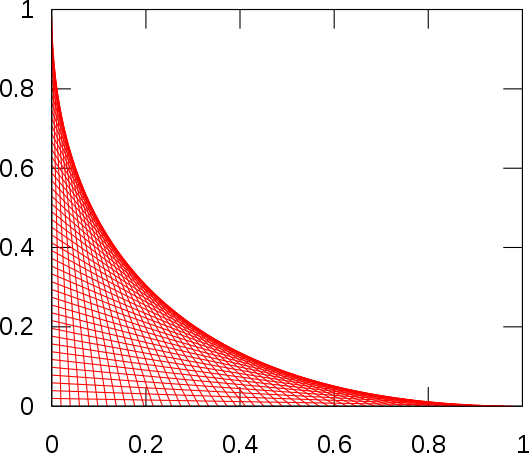
\includegraphics{envelope.png}
	\labfig{margin2}
\end{marginfigure}
Así tenemos dos nuevas coordenadas $[p,g(p)]$, relacionadas con $[x,f(x)]$ mediante
\vspace{-5pt}
\begin{equation} \label{4.1.1}
    \begin{matrix}
        p(x)=f'(x) && \color{blue}g(p)\color{black}=f(x(p))-x(p)\color{blue}p\color{black} &&[x,f(x)] \mapsto [p,g(p)] \\
        x(p)=(f')^{-1}(p) &&  \color{blue}f(x) \color{black}=p(x)\color{blue}x\color{black}+g(p(x))  && [p,g(p)] \mapsto [x,f(x)]\
    \end{matrix}
\end{equation} \refstepcounter{subsection}
Donde la primera expresión es la \textit{Transformada de Legendre}, y será invertible (la segunda expresión) siempre que $f'(x)$ sea invertible (cierto si $f''(x)\neq 0$).
\subsection{Varias variables}
Si ahora tenemos $f(\{x_i,y_i\})$ donde $\{y_i\}$ son las variables sobre las que queremos hacer la transformada, la transformada es entonces
\begin{equation} \label{4.1.2}
    \begin{matrix}
        p_i(\{x_i,y_i\})=\frac{\partial f}{\partial y_i} && g(\{x_i,\color{blue}p_i\color{black}\}) =f(\{x_i,y_i(\{x_i,p_i\})\}) -\sum_j \color{blue}p_j\color{black} y_j(\{x_i,p_i\})  &&[y_i,f] \mapsto [p_i,g] \\
        y_i(\{x_i,p_i\})=\left[\frac{\partial f}{\partial y_i}\right]^{-1} && f(\{x_i,\color{blue}y_i\color{black}\}) =\sum_j \color{blue}y_j\color{black} p_j (\{x_i,y_i\})  +g(\{x_i,p_i(\{x_i,y_i\})\}) &&[p_i,g] \mapsto [y_i,f]\\
    \end{matrix}
\end{equation} \refstepcounter{subsection}
La transformación será inversible si el jacobiano de $y_i \mapsto p_i$ es no nulo.
\subsubsection{Transformada de Legendre del Lagrangiano}
Ahora si tenemos $\pazocal{L}(\{q_j,\dot{q}_j\};t)$, $\{\dot{q}_j\}$ serán nuestras antiguas variables y las nuevas variables serán $\partial_{\dot{q}_j}\pazocal{L}=p_j$, los momentos generalizados o conjugados. Entonces aplicando (4.1.2) llegamos a (3.1.2)
\begin{equation} \label{4.1.3}
        p_i(\{q_i,\dot{q}_i\};t)=\frac{\partial \pazocal{L}}{\partial q_i} \ \ \ \ \ \  g(\{q_i,p_i\};t) =\pazocal{L}(\{q_i,p_i\};t) -\sum_j^s \dot{q}_j (\{q_i,p_i\}) p_j = -\pazocal{H}
\end{equation} \refstepcounter{subsection}
De esta forma, $\pazocal{H}$ es equivalente a la \textit{Transformada de Legendre} de $\pazocal{L}$ con respecto a los $\dot{q}_j$, y esta es inversible, la demostración de que el jacobiano $[\partial_{\dot{q}_j}p_i]$ es no nulo bajo ciertas circumstancias se deja como un ejercicio al lector.

De esta forma, no hemos perdido ninguna información del sistema al pasar de $\pazocal{L}$ a $\pazocal{H}$, y a continuación reformularemos las ecuaciones del movimiento en función de esta cantidad de una forma equivalente a la fomulación lagrangiana.
\section{Ecuaciones de Hamilton} \refstepcounter{subsection}
Si hacemos la diferencial exacta de $\pazocal{H}$ usando la regla de la cadena tenemos
\begin{equation} \label{4.2.1}
    d\pazocal{H} = \sum^s\left(\frac{\partial \pazocal{H}}{\partial q_j}dq_j+\frac{\partial \pazocal{H}}{\partial p_j}dp_j\right)+\frac{\partial \pazocal{H}}{\partial t} dt
\end{equation} \refstepcounter{subsection}
Si por otro lado hacemos el diferencial de $\pazocal{H}$ desde (3.1.2) o (4.1.3)
\begin{equation} \label{4.2.2}
    d\pazocal{H} = \sum^s\left(p_j d\dot{q}_j+\dot{q}_j dp_j\right)-d\pazocal{L}
\end{equation} \refstepcounter{subsection}
si $d\pazocal{L}$ es por regla de la cadena, y usando (2.2.1) y (2.2.2)
\begin{equation} \label{4.2.3}
    d\pazocal{L}= \sum^s\left(\frac{\partial \pazocal{L}}{\partial q_j}dq_j+\frac{\partial \pazocal{L}}{\partial \dot{q}_j}d\dot{q}_j\right) + \frac{\partial \pazocal{L}}{\partial t}dt = \sum^s\left(\dot{p}_j dq_j+p_j d\dot{q}_j\right) + \frac{\partial \pazocal{L}}{\partial t}dt
\end{equation} \refstepcounter{subsection}
Sustituyendo (4.2.3) en (4.2.2)
\begin{equation} \label{4.2.4}
    d\pazocal{H} = \sum^s p_j d\dot{q}_j+\dot{q}_j dp_j-\sum^s \dot{p}_j dq_j+p_j d\dot{q}_j - \frac{\partial \pazocal{L}}{\partial t}dt = \sum^s \dot{q}_j dp_j-\dot{p}_j dq_j - \frac{\partial \pazocal{L}}{\partial t}dt
\end{equation} \refstepcounter{subsection}
Como $dq_j$, $dp_j$ y $dt$ son funciones independientes y arbitrarias, podemos igualar término a término (4.2.4) y (4.2.1), de tal forma que obtenemos tres ecuaciones
\Large \begin{equation} \label{4.2.5}
    \boxed{\dot{q}_j = \frac{\partial \pazocal{H}}{\partial p_j} \ \ \ \ \ \ \dot{p}_j= -\frac{\partial \pazocal{H}}{\partial q_j}}
\end{equation} \refstepcounter{subsection} \normalsize
Estas dos primeras ecuaciones son las \textit{Ecuaciones de Hamilton} del movimiento o \textit{Ecuaciones canónicas}. Por otro lado tenemos la tercera ecuación, que junto a (3.1.2)
\begin{equation} \label{4.2.6}
    \frac{\partial \pazocal{H}}{\partial t} = - \frac{\partial \pazocal{L}}{\partial t} = \frac{d \pazocal{H}}{dt}
\end{equation} \refstepcounter{subsection}
De esta forma, si $\pazocal{H}$ no depende explícitamente del tiempo, este se conserva.

Para aplicar estas ecuaciones en un sistema holonómico tenemos que hayar primero $\pazocal{L}$, tras esto hallar los momentos generalizados y despues invertir la relación, tal que
\begin{equation} \label{4.2.7}
    p_j = \frac{\partial \pazocal{L}}{\partial \dot{q}_j}=p_j(\{q_k,\dot{q}_k\};t) \rightarrow \dot{q}_j = \dot{q}_j(\{q_k,p_k\};t)
\end{equation} \refstepcounter{subsection}
Entonces usamos la ecuación (4.1.3) con mucho cuidado de reemplazar todas las $\dot{q}_j$ por (4.2.7), y ya tendremos $\pazocal{H}$ en una forma que nos permita resolverlo usando (4.2.5).

Además, usando (4.1.3) podemos escribir $\pazocal{L}$ como
\begin{equation} \label{4.2.7}
    \pazocal{L}(\{q_i,p_i\};t) = \sum_j^s p_j \dot{q}_j (\{q_i,p_i\};t) -\pazocal{H}(\{q_i,p_i\};t)
\end{equation} \refstepcounter{subsection}
Si hacemos la acción de ese lagrangiano tendremos, y al extremizarla se puede comprobar que se obtienen (4.2.5)
\begin{equation} \label{4.2.7}
    S = \int_{t_A}^{t_B} \left(\sum_j^s p_j \dot{q}_j -\pazocal{H}\right) dt
\end{equation} \refstepcounter{subsection}
Para ello, aplicamos los metodos explicados en el Capítulo 1, teniendo en cuenta que $\pazocal{L}$ no depende de $\dot{p}_i$ 
\[
    \delta S = 0 = \int_{t_A}^{t_B} \delta \pazocal{L} dt = \int_{t_A}^{t_B} \sum_i\left(\frac{\partial \pazocal{L}}{\partial q_i} \delta q_i + \frac{\partial \pazocal{L}}{\partial \dot{q}_i} \delta \dot{q}_i + \frac{\partial \pazocal{L}}{\partial p_i} \delta p_i\right) dt
\]
Integrando el segundo término por partes como en (1.2.1), usando que $\delta \dot{q}_i =  \dot{(\delta q_i)}$
\[
    \delta S = 0 = \int_{t_A}^{t_B} \sum_{i}\left[\left(\frac{\partial \pazocal{L}}{\partial q_i} - \frac{d}{dt}\left(\frac{\partial \pazocal{L}}{\partial \dot{q}_i}\right)\right) \delta q_i + \frac{\partial \pazocal{L}}{\partial p_i}\delta p_i\right] dt
\]
Haciendo las derivadas de $\pazocal{L}$ obtenemos
\[
    \delta S = 0 = \int_{t_A}^{t_B} \sum_{i}\left[\left(-\frac{\partial \pazocal{H}}{\partial q_i} - \dot{p}_i\right) \delta q_i + \left(\dot{q}_i-\frac{\partial \pazocal{H}}{\partial p_i}\right)\delta p_i\right] dt
\]
Y ahora, establecemos que los términos entre paréntesis deben ser 0, puesto que las variaciones son arbitrarias e independientes, obteniendo (4.2.5).
\vspace{-20pt}
\subsubsection{Ejemplo}
Un ejemplo sencillo es el péndulo simple donde 
\[\pazocal{L}=\frac{1}{2}ml^2\dot{\theta}^2+mgl\cos{\theta} \ \ \ \ \ \ p_\theta = \frac{\partial \pazocal{L}}{\partial \dot{\theta}}=ml^2\dot{\theta} \ \ \ \ \ \ \dot{\theta}=\frac{p_\theta}{ml^2}=\dot{\theta}(p_\theta)\]
Sustituyendo tenemos 
\[\pazocal{H}=p_\theta \dot{\theta} -\pazocal{L}=\frac{p_\theta^2}{ml^2} - \frac{p_\theta^2}{2ml^2}-mgl\cos\theta = \frac{p_\theta^2}{2ml^2}-mgl\cos\theta = T+U\]

Ahora aplicamos (4.2.5.A), tal que $\dot{\theta} = p_\theta/ml^2$, de donde sacamos que $\dot{p}_\theta=ml^2 \ddot{\theta}$ y de (4.2.5.B) sacamos $\dot{p}_\theta=-mgl\sin\theta$, igualando y depejando tenemos $\ddot{\theta} + g/l \sin\theta = 0$, la ecuación del movimiento.
\subsubsection{Comparación Lagrange-Hamilton}
La formulación Lagrangiana es mejor para tratar con ligaduras, pero la hamiltoniana nos permite reducir el orden de la ecuación diferencial resultante cuando no hay dependencia explícita en una o varias de las $q_j$, puesto que en (3.1.5) $  \pazocal{L}$ sigue dependiendo de $\dot{q}_j$, solo conseguimos reducir en 1 el orden de un ecuación de E-L, mientras que en la formulación hamiltoniana, si una variable es cíclica, es decir $\partial_{q_j}\pazocal{H}=0$, entonces ya hemos resuelto $p_j=\alpha$ por (4.2.5.B) y también por definición $\pazocal{H}$ no depende de $q_j$, de esta forma nos hemos eliminado dos dependencias y reducir el orden en 2 unidades, podemos integrar $q_j$ usando (4.2.5.A) que como no depende de $q_j$ es una EDO separable. 
\section{Espacio de fase} \refstepcounter{subsection}
El hecho de que solo haya una sola solución para las ecuaciones del movimiento, es decir, que solo hay una posible trayectoria dadas unas condiciones dadas, significa que el sistema con el que estamos tratando es \textit{determinista}.

Si es el espacio de configuración es $\{q_j\}$ para un $t$ dado, entonces definimos el \textbg{Espacio de fase} como $\{q_j,p_j\}$, donde $\{p_j\}$ es el espacio de momentos o impulsos.

Este espacio es de dimensión $2s$ y nos da toda la información dinámica del sistema pues nos permite predecir su evolución, puesto que con unas condiciones iniciales de posición y momento (o velocidad) definidas por unas coordendas del espacio de fase, podemos usar (4.2.5) (Ecs. H.) para hallar la evolución del sistema.

\subsection{Diagrama de fases}
Es la trayectoria que sigue un sistema en el espacio de fase, normalmente representada en un conjunto de $s$ planos bidimensionales como una curva en cada uno de ellos, cuyos ejes representan $q_j$ y $p_j$, donde por cada punto en un $t$ dado solo puede pasar una sola trayectoria, de lo contrario el sistema no sería determinista, ya que de unas mismas condiciones iniciales podría evolucionar de varias formas.

Además si $\pazocal{H}$ se conserva, entonces por cada punto del espacio de fase solo puede pasar una trayectoria independientemente del tiempo.

\subsubsection{Ejemplo}
\begin{marginfigure}[0cm]
	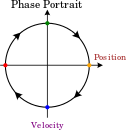
\includegraphics{phase.png}
	\labfig{margin3}
\end{marginfigure}
Como ejemplo vamos a ver un péndulo, tomando las expresiones del ejemplo de (4.2), donde las coordenadas del espacio de fases son $(\theta,p_\theta)$, si $\theta << 1$, tenemos $\ddot{\theta}+\frac{g}{l}\theta=0$, cuya solución, donde $\omega^2=g/l$, es
\[\theta = A \sin{(\omega t + \theta_0)}+ B \cos{(\omega t + \theta_0)} \ \ \ \ \dot{\theta} = A\omega \cos{(\omega t + \theta_0)}- B \omega \sin{(\omega t + \theta_0)} \ \ \ \ p_\theta = ml^2 \dot{\theta}\]
\[\theta^2 + \frac{p_\theta^2}{\omega^2 m^2l^4}=A^2+B^2 \mbox{ (elipse)}\]
\subsection{Teorema de Liouville} \refstepcounter{subsection}
\subsubsection{Volumen en el espacio de fase}
Definimos el volumen en el espacio de fases como
\begin{equation} \label{4.3.1}
    V = \prod_j^s \Delta q_j \Delta p_j
\end{equation} \refstepcounter{subsection}
Donde $\Delta q_j \Delta p_j$ es el área en uno de los $s$ planos.

Si ahora tenemos una serie de condiciones iniciales distribuidas dentro de una región volumétrica del espacio de fases, siendo $\pazocal{N}$ el número de condiciones iniales dentro de $V$, entonces si consideramos como la frontera de $V$ se transforma con el tiempo para dar $V'$, entonces $\pazocal{N}$ se conserva, puesto que para que una trayectoria entre o salga del volumen sería necesario que cortase una trayectoria de la frontera, lo cual no puede ocurrir en un sistema determinista.
\subsubsection{Teorema de Liouville} \refstepcounter{subsection}
El volumen $V(S)$ dentro de una superficie $S(t)$ del espacio de fase se conserva.
\begin{equation} \label{4.3.2}
    \frac{dV}{dt}=0 \implies \frac{d\rho}{dt} = 0 \ \ \ \ \rho = \frac{\pazocal{N}}{V}
\end{equation} \refstepcounter{susection}

\textbf{Demostración intuitiva}

Sean $\mathbf{z}=(\mathbf{q},\mathbf{p})$, $\mathbf{v}=\dot{\mathbf{z}}=(\dot{\mathbf{q}},\dot{\mathbf{p}})$, y $\mathbf{\nabla} = (\mathbf{\nabla}_\textbf{q},\mathbf{\nabla}_\textbf{p})$, entonces la divergencia de $\mathbf{v}$, tal que
\begin{equation} \label{4.3.4}
    \mathbf{\nabla} \cdot \mathbf{v} = \sum^s \frac{\partial \dot{q}_j}{\partial q_j} + \frac{\partial \dot{p}_j}{\partial p_j}
\end{equation} \refstepcounter{subsection}
entonces por el Teorema de la Divergencia
\begin{equation} \label{4.3.5}
    \int_V{\mathbf{\nabla} \cdot \mathbf{v} dV} = \int_S \mathbf{v} \cdot d\mathbf{S}
\end{equation} \refstepcounter{subsection}
La variación de $V$ en términos del tiempo es la siguiente, ya que $\mathbf{v}dt$ indica como se mueven las partículas de dentro de $V$, y multiplicando por $d\mathbf{S}$ nos indica como varía el volumen infinitesimalmente en un punto de la superficie, integrando en la superficie para ver la variación total de $V$ tenemos
\begin{equation} \label{4.3.6}
    dV=\int_S \mathbf{v} \cdot d\mathbf{S} dt \implies \frac{dV}{dt} = \int_S \mathbf{v} \cdot d\mathbf{S}
\end{equation} \refstepcounter{subsection}
Combinando (4.4.4), (4.4.5) y sustituyendo (4.4.3) llegamos a 
\begin{equation} \label{4.3.7}
    \frac{dV}{dt} = \int_V{\mathbf{\nabla} \cdot \mathbf{v} dV} = \int_V{\left(\sum^s \frac{\partial \dot{q}_j}{\partial q_j} + \frac{\partial \dot{p}_j}{\partial p_j}\right)dV}
\end{equation} \refstepcounter{subsection}
Ahora usando (4.2.5) (Ecs. H.) y que las parciales conmutan.
\begin{equation} \label{4.3.8}
    \frac{dV}{dt} = \int_V{\left(\sum^s \frac{\partial \pazocal{H}}{\partial q_j p_j} - \frac{\partial \pazocal{H}}{\partial p_j q_j}\right)dV} = 0
\end{equation} \refstepcounter{subsection}
\section{Paréntesis de Poisson} \refstepcounter{subsection}
Sea $f=f(\{q_j,p_j\};t)$ una función de las coordenadas canónicas, podemos hacer su derivada total con respecto al tiempo, tal que
\begin{equation} \label{4.4.1}
    \frac{d f}{dt} = \sum^s \left(\frac{\partial f}{\partial q_j}\dot{q}_j+\frac{\partial f}{\partial p_j}\dot{p}_j\right) + \frac{\partial f}{\partial t}
\end{equation} \refstepcounter{subsection}
Usando (3.2.5) (Ecs. H.) llegamos a 
\begin{equation} \label{4.4.2}
\frac{d f}{dt} = \sum^s \left(\frac{\partial f}{\partial q_j}\frac{\partial \pazocal{H}}{\partial p_j}-\frac{\partial f}{\partial p_j}\frac{\partial \pazocal{H}}{\partial q_j}\right) + \frac{\patial f}{\partial t} = [f,\pazocal{H}] + \frac{\partial f}{\partial t}
\end{equation} \refstepcounter{subsection}
Dónde $[f,\pazocal{H}]$ es el \textit{paréntesis de Poisson} de $f$ y $\pazocal{H}$, en general lo definimos para dos funciones como
\begin{equation} \label{4.4.3}
    [f,g]=  \sum^s \left(\frac{\partial f}{\partial q_j}\frac{\partial g}{\partial p_j}-\frac{\partial f}{\partial p_j}\frac{\partial g}{\partial q_j}\right)
\end{equation} \refstepcounter{subsection}
Sus propiedades algebraicas son muy similares a aquellas del producto vectorial puesto que su expresión es muy similar, son sencillas de verificar reemplando a fuerza bruta en (4.4.3).
\begin{itemize}
    \item Es alternada $[f,g]=-[g,f]$ y $[f,f]=0$.
    \item Si $[f,g]=0 \iff [f,g]=[g,f]=0$ las funciones conmutan.
    \item Es bilineal, $[f,\alpha g + \beta h] = \alpha [f,g] + \beta [f,h]$.
    \item Existe una regla del producto $[f,gh]=g[f,h]+h[f,g]$.
    \item Se verifica la \textit{Identidad de Jacobi}, $\left[f,[g,h]\right]+\left[h,[f,g]\right]+\left[g,[h,f]\right]=0$.
\end{itemize}
Otra regla del producto que se verifica, usando la conmutividad de las derivadas parciales, es $\frac{\partial}{\partial t}[f,g]=[\frac{\partial f}{\partial t},g]+[f,\frac{\partial g}{\partial t}]$.

Si la función $f$ no depende explícitamente del tiempo, entonces si $f$ conmuta con $\pazocal{H}$, eso implica por (4.4.2) y las propiedades anteriores, que $f$ se conserva.

Además, si tenemos dos cantidades conservadas $f$ y $g$, entonces tenemos que, usando la \textit{Identidad de Jacobi}, se conserva su paréntesis
\begin{equation} \label{4.4.5}
    \frac{d}{dt}[f,g]=0
\end{equation}

Si hacemos $[q_k,\pazocal{H}]$ y $[p_k,\pazocal{H}]$ aplicando (4.4.3) y (3.2.5) (Ecs. H.), obtenemos las ecuaciones del movimiento expresadas en términos de \textit{paréntesis de Poisson}.
\begin{equation} \label{4.4.6}
    \boxed{[q_k,\pazocal{H}] = \dot{q}_k \ \ \ \ \ [p_k,\pazocal{H}]=\dot{p}_k}
\end{equation}
Tenemos también los paréntesis de \textit{paréntesis de Poisson} fundamentales
\begin{equation} \label{4.4.7}
    [q_k,q_l]=[p_k,p_l]=0 \ \ \ \ \ [q_k,p_l]=\delta_{kl}
\end{equation}
En mecánica cuántica se define un operador similar, y expresar expresar sistemas en términos de \textit{paréntesis de Poisson} nos permite cuantizarlos. Un ejemplo es que (4.4.2) se convierte en la ecuación de \textit{Heissenberg}.

No hay mucho detalle en esta sección por que no es muy relevante para este curso, se incluye para familiarizarse con este formalismo.


%----------------------------------------------------------------------------------------

\backmatter % Denotes the end of the main document content
\end{document}
